\chapter{Simulation results}
\label{chap: results}

In this chapter we present the work done in order to validate the numerical implementation of the discretization method illustrated in Chapter \ref{chap: finite element}, in FEMOS 3D code compared with a reference simulation tool (SDEVICE, commercialized by Synopsis \cite{SdeviceManual}).
In particular we illustrate (and compare) the algorithm used to calculate the current at the ohmic contacts.

\section{Test cases}

We consider three kinds of semiconductor devices: 

\begin{itemize}
\setlength{\itemsep}{0.5pt}
\item {\bf p-n junction}
\item {\bf p-n junction in oxide}
\item {\bf n-channel / p-channel MOSFET}
\end{itemize}

\subsection{p-n junction}
\label{sec: PN}

In this example we consider a simple p-n junction. \figref{fig: diodo struttura} presents the partition and the doping profile for this test. The section of the parallelepiped is a $0.05 \times 0.05 [\mu m^2]$ square while the device is $0.1 [\mu m]$ long.  The number of vertices are $4933$, while the elements are $24576$.  The doping concentration is obtained setting a constant profile of acceptors over all the domain ($N_A^- = 1.0\times 10^{17} [cm^{-3}]$) overwhelmed by a doping profile of  donors ($N_D^+=1.0 \times 10^{18} [cm^{-3}]$) bounded on one side of the device and resulting in an almost abrupt junction. 
Two contacts are defined: (A) contact is placed at $Z=0.1[\mu m]$ and (B) contact is placed at $Z=0.0 [\mu m]$.  


\begin{figure}[!t]
\centering
\subfloat[][\emph{Mesh.}]
{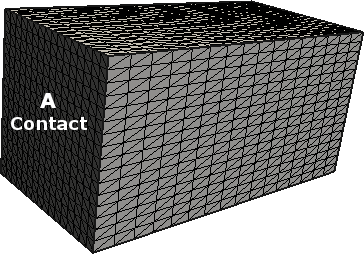
\includegraphics[width=0.35\textwidth , height=3.0cm]{Results/DIODE/AAA_structureandcontactFINITO.png}}
\hspace{0.06\textwidth}
\subfloat[][\emph{Doping concentration.}]
{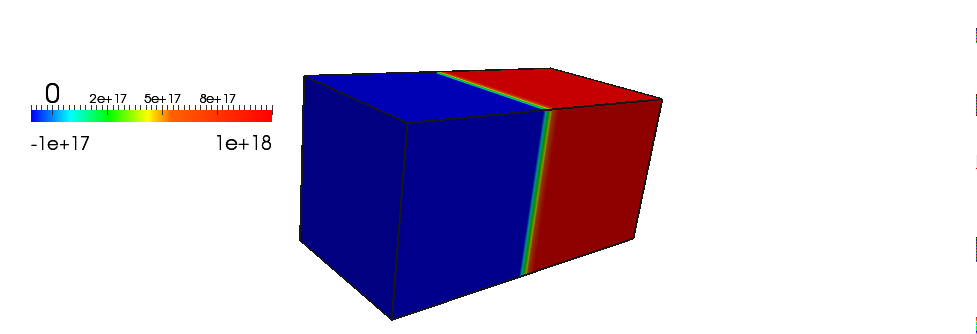
\includegraphics[width=0.35\textwidth ,  height=3.0cm]{Results/DIODE/AAA_Dopingconcentration.png}}
\hspace{0.04\textwidth}
{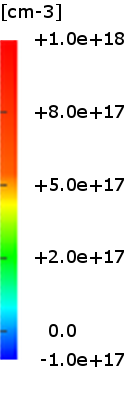
\includegraphics[width=0.1\textwidth ,  height=3.4cm]{Results/DIODE/LegendDopingDiode.png}}
\caption{p-n junction.}
\label{fig: diodo struttura}
\end{figure}


In order to analyze the operating function of the diode, two cases of direct bias are performed: $0.3[V]$-$1.0[V]$. The setting values and the parameters are summarized in \tabref{tab: diode direct}. 
\figref{fig: Solutions case test 0.3} reports the solutions for $V_A=0.3[V]$ and $V_A=1.0[V]$, along a line parallel to the Z-axis and placed at the center of the device. 
Because the built-in voltage is around $0.7 \div 0.8 [V]$ the behaviour of the device is different when the applied bias is below or above this threshold. 
At a bias voltage of $0.3[V]$, potential drop is almost bounded around the junction, and due to the asymmetric doping, is mostly extended in the p-side. Carriers cannot cross the potential barrier and this causes low current flux inside the device.
At $1.0[V]$ the minority carrier density becomes almost ten order bigger, resulting in a large amount of current toward the contacts:  the device turns from exponential to linear resistive. This is clear in \figref{fig: diode 1v pot} where the potential shape becomes similar to a that of a resistance voltage profile (linear potential profile). Comparing the quasi Fermi potentials of \figref{fig: qf pot diode 03} and \figref{fig: qf pot diode 1} the boundary layers at contacts increase with the applied bias. This effect is related to the ohmic contact hypothesis, and can be changed by adopting different boundary condition: this occurs also for the carrier concentration because at the contacts, charge neutrality and thermodynamic equilibrium  are imposed.

\figsref{fig: diode potential 03V}-\ref{fig: pdensity 03V} show the comparison between SDEVICE and FEMOS in 3D plots for electrostatic potential, electron and hole densities at $0.3[V]$, while \figsref{fig: diode potential 1V}-\ref{fig: pdensity 1V} show the same comparison at $1.0[V]$. In both conditions the agreement is very good.

\begin{table}[!h]
\centering
\begin{tabular}{cccc}
\toprule
 Test case $[V]$  & Mobility model $[cm^2V^{-1}s^{-1}]$  & R/G model & $\epsilon_{Si}$\\
\midrule
$V_A=0.3$ & $\mu_n = 1417$, $\mu_p = 470.5$ & SRH, Auger & 11.6 \\
$V_A=1.0$ & $\mu_n = 1417$, $\mu_p = 470.5$ & SRH, Auger & 11.6 \\\bottomrule
\end{tabular}
\caption{p-n junction - list of settings, parameters and models.}
\label{tab: diode direct}
\end{table}


\begin{figure}[!h]
\centering

\subfloat[][\emph{Potential}]
{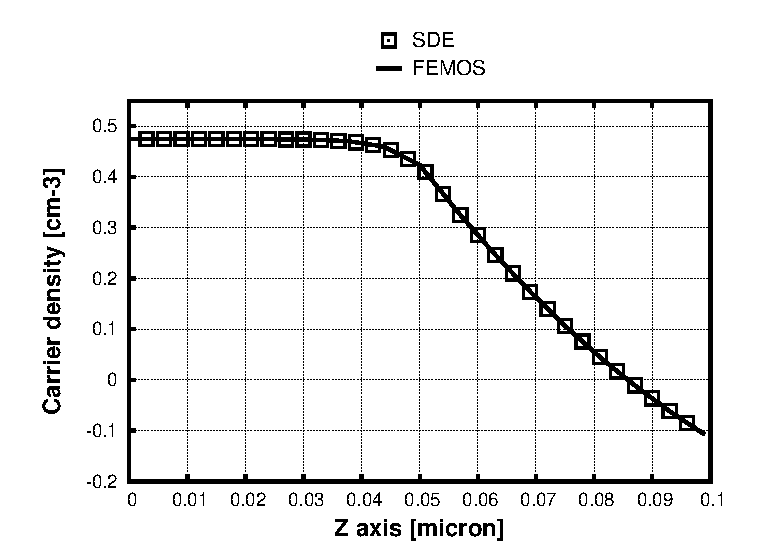
\includegraphics[width=0.5\textwidth , height=5cm]{DatiImmaginiTESI/Diode/PotentialZaxis03volt.eps}}
\subfloat[][\emph{Potential} \label{fig: diode 1v pot}]
{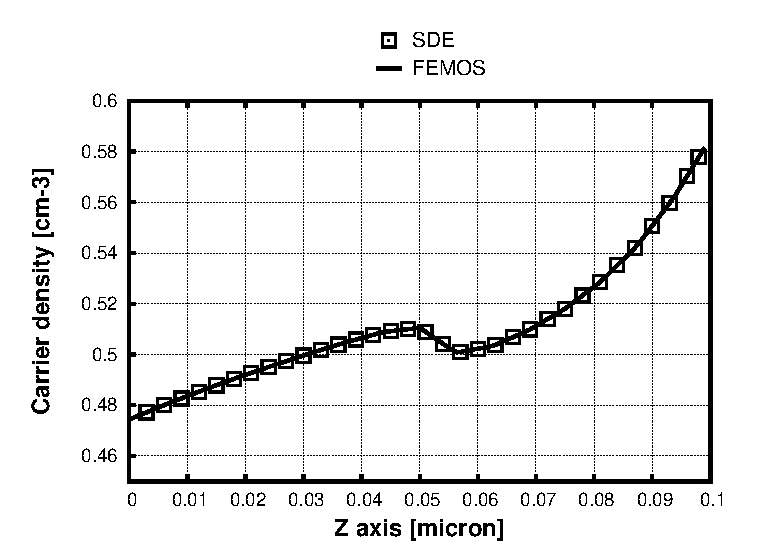
\includegraphics[width=0.5\textwidth , height=5cm]{DatiImmaginiTESI/Diode/PotentialZaxis1volt.eps}}


\subfloat[][\emph{Carriers}]
{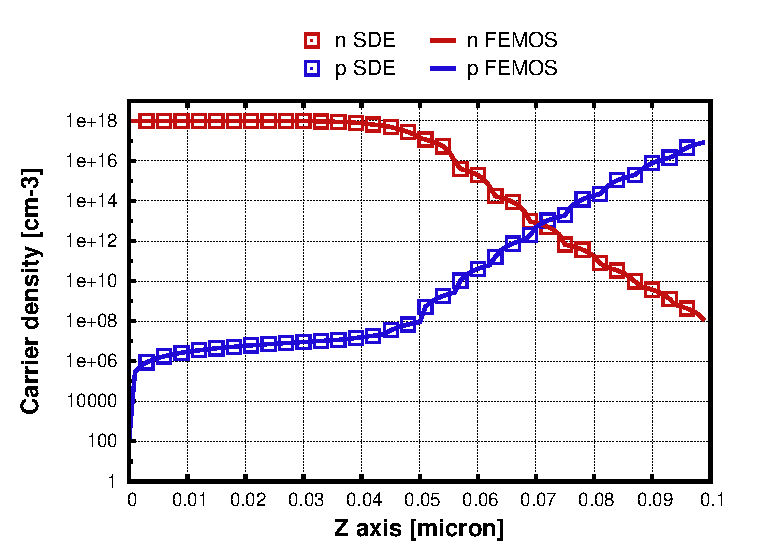
\includegraphics[width=0.5\textwidth , height=5cm]{DatiImmaginiTESI/Diode/DensitiesZaxis03volt.eps}}
\subfloat[][\emph{Carriers}]
{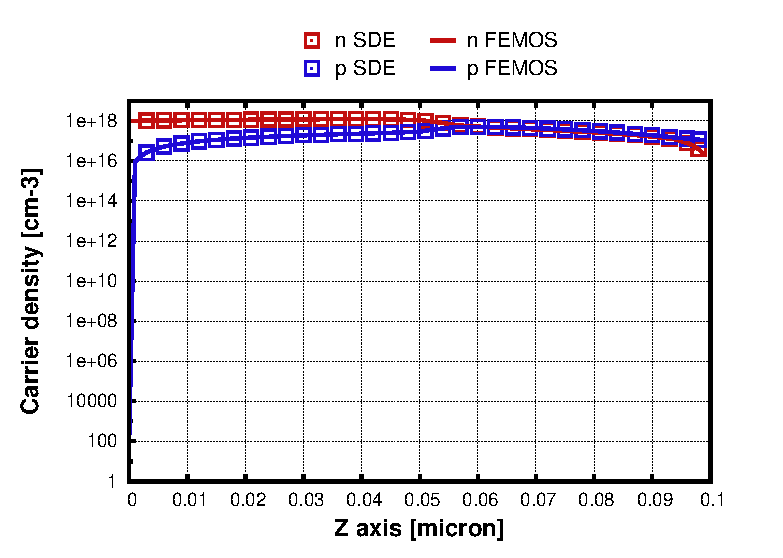
\includegraphics[width=0.5\textwidth , height=5cm]{DatiImmaginiTESI/Diode/DensitiesZaxis1volt.eps}}


\subfloat[][\emph{Quasi Fermi potentials} \label{fig: qf pot diode 03}]
{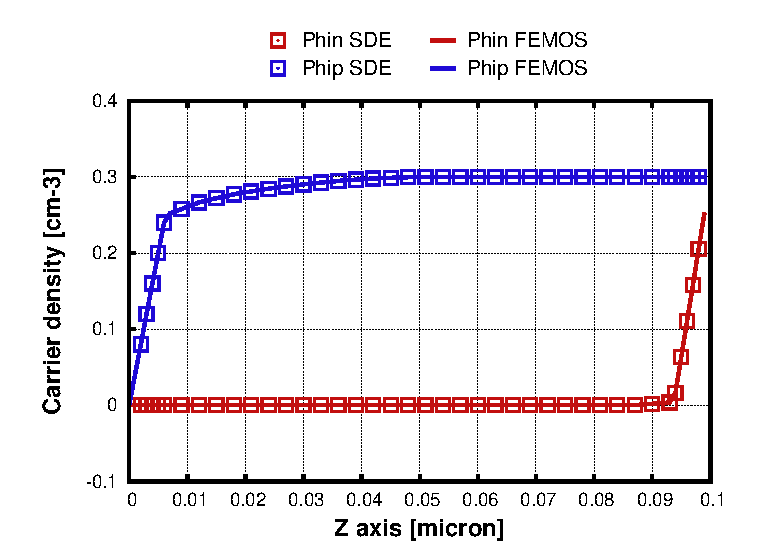
\includegraphics[width=0.5\textwidth , height=5cm]{DatiImmaginiTESI/Diode/QuasiFermiZaxis03volt.eps}}
\subfloat[][\emph{Quasi Fermi potentials} \label{fig: qf pot diode 1}]
{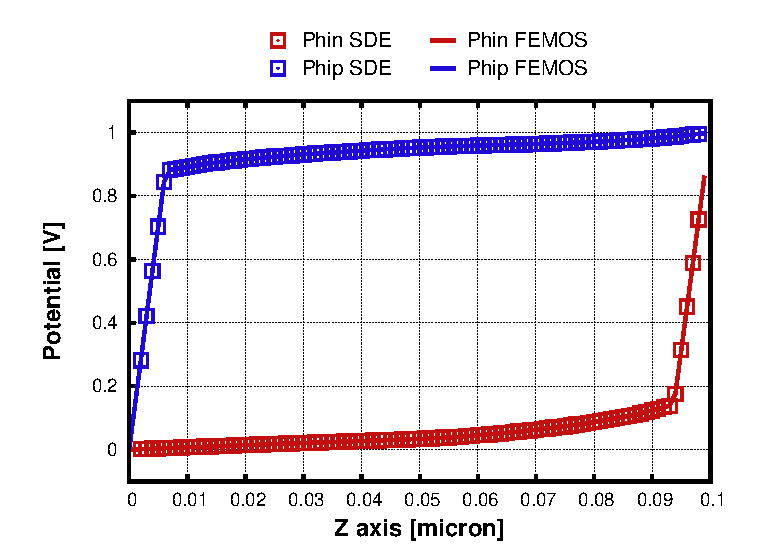
\includegraphics[width=0.5\textwidth , height=5cm]{DatiImmaginiTESI/Diode/QuasiFermiZaxis1volt.eps}}

\caption{1D plots of the solutions and the quasi fermi potential levels along the line parallel to the Z-axis and placed at the center of the device of \figref{fig: diodo struttura}. On the left is presented the test case at $V_A=0.3[V]$ while on the right at $V_A=1.0[V]$.}
\label{fig: Solutions case test 0.3}
\end{figure}


\clearpage 

\begin{figure}[!h]
\centering
\subfloat[][\emph{FEMOS}]
{\includegraphics[width=0.38\textwidth , height=3.7cm]{Results/DIODE/FEMOS1817_potential03volt.png}}
\hspace{0.06\textwidth}
\subfloat[][\emph{SDEVICE}]
{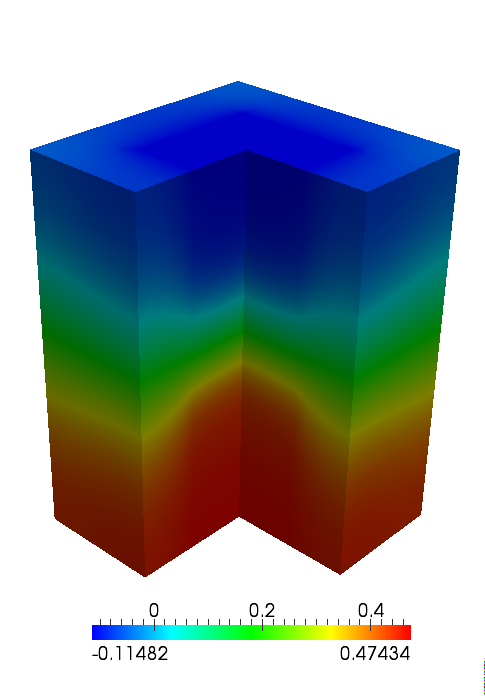
\includegraphics[width=0.38\textwidth , height=3.7cm]{Results/DIODE/SDEVICE1817_potential03volt.png}}
\hspace{0.04\textwidth}
{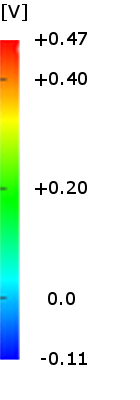
\includegraphics[width=0.1\textwidth , height=3.7cm]{Results/DIODE/LegendPotentialDiode03volt.png}}
\caption{p-n junction 0.3[V] - Electrostatic Potential.}
\label{fig: diode potential 03V}
\end{figure}


\vspace{1cm}

\begin{figure}[!h]
\centering
\subfloat[][\emph{FEMOS}]
{\includegraphics[width=0.38\textwidth , height=3.7cm]{Results/DIODE/FEMOS1817_edensity03volt.png}}
\hspace{0.06\textwidth}
\subfloat[][\emph{SDEVICE}]
{\includegraphics[width=0.38\textwidth , height=3.7cm]{Results/DIODE/FEMOS1817_edensity03volt.png}}
\hspace{0.04\textwidth}
{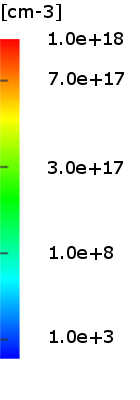
\includegraphics[width=0.1\textwidth , height=3.7cm]{Results/DIODE/LegendEdensityDiode03volt.png}}
\caption{p-n junction 0.3[V] -  Electron density.}
\label{fig: ndensity 03V}
\end{figure}

\vspace{1cm}

\begin{figure}[!h]
\centering
\subfloat[][\emph{FEMOS}]
{\includegraphics[width=0.38\textwidth , height=3.7cm]{Results/DIODE/FEMOS1817_hdensity03volt.png}}
\hspace{0.06\textwidth}
\subfloat[][\emph{SDEVICE}]
{\includegraphics[width=0.38\textwidth , height=3.7cm]{Results/DIODE/FEMOS1817_hdensity03volt.png}}
\hspace{0.04\textwidth}
{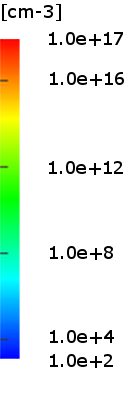
\includegraphics[width=0.1\textwidth , height=3.7cm]{Results/DIODE/LegendHdensityDiode03volt.png}}
\caption{p-n junction 0.3[V] - Hole density.}
\label{fig: pdensity 03V}
\end{figure}


\clearpage

\begin{figure}[!h]
\centering
\subfloat[][\emph{FEMOS}]
{\includegraphics[width=0.38\textwidth , height=3.7cm]{Results/DIODE/FEMOS1817_potential1voltONLYDEVICE.png}}
\hspace{0.06\textwidth}
\subfloat[][\emph{SDEVICE}]
{\includegraphics[width=0.38\textwidth , height=3.7cm]{Results/DIODE/FEMOS1817_potential1voltONLYDEVICE.png}}
\hspace{0.04\textwidth}
{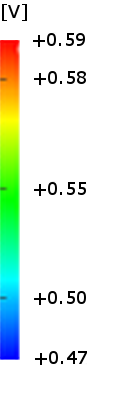
\includegraphics[width=0.1\textwidth , height=3.7cm]{Results/DIODE/LegendPotentialDiode1volt.png}}
\caption{p-n junction 1.0[V] - Electrostatic Potential.}
\label{fig: diode potential 1V}
\end{figure}

\vspace{1cm}

\begin{figure}[!h]
\centering
\subfloat[][\emph{FEMOS}]
{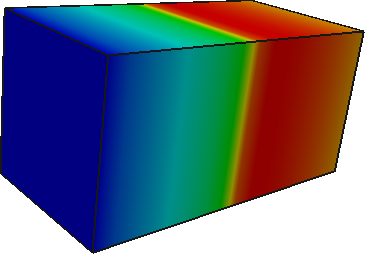
\includegraphics[width=0.38\textwidth , height=3.7cm]{Results/DIODE/FEMOS1817_edensity1voltLINEARONLYDEVICE.png}}
\hspace{0.06\textwidth}
\subfloat[][\emph{SDEVICE}]
{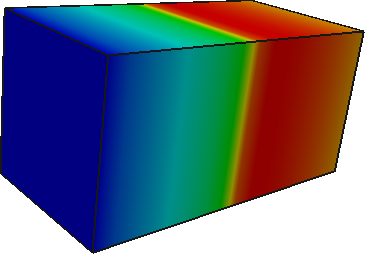
\includegraphics[width=0.38\textwidth , height=3.7cm]{Results/DIODE/FEMOS1817_edensity1voltLINEARONLYDEVICE.png}}
\hspace{0.04\textwidth}
{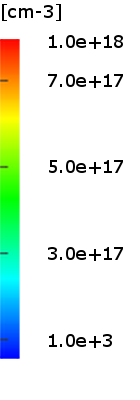
\includegraphics[width=0.1\textwidth , height=3.7cm]{Results/DIODE/LegendEdensityDiode1volt.png}}
\caption{p-n junction 1.0[V] -  Electron density.}
\label{fig: ndensity 1V}
\end{figure}

\vspace{1cm}

\begin{figure}[!h]
\centering
\subfloat[][\emph{FEMOS}]
{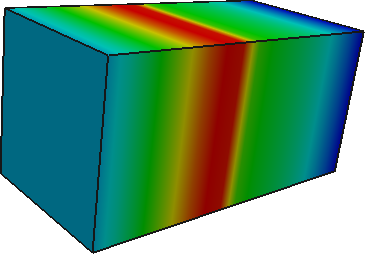
\includegraphics[width=0.38\textwidth , height=3.7cm]{Results/DIODE/FEMOS1817_hdensity1voltLINEARONLYDEVICE.png}}
\hspace{0.06\textwidth}
\subfloat[][\emph{SDEVICE}]
{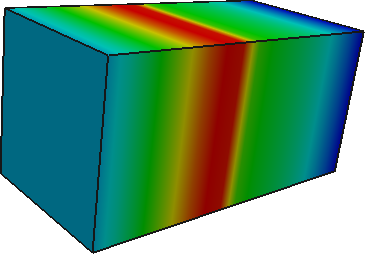
\includegraphics[width=0.38\textwidth , height=3.7cm]{Results/DIODE/FEMOS1817_hdensity1voltLINEARONLYDEVICE.png}}
\hspace{0.04\textwidth}
{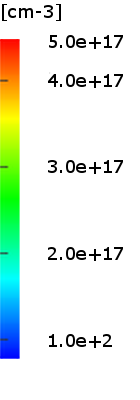
\includegraphics[width=0.1\textwidth , height=3.7cm]{Results/DIODE/LegendHdensityDiode1volt.png}}
\caption{p-n junction 1.0[V] - Hole density.}
\label{fig: pdensity 1V}
\end{figure}

\clearpage

\subsubsection{Computational cost and initial condition}

Computational experience demonstrates that convergence of the Gummel algorithm is strictly related to the kind of chosen initial condition: the closest to solution, the better the convergence. However, to predict in every situation the possible shape of the solutions is hard (if not even impossible). For this reason we have adopted a common and general approach splitting the domain in several regions according to their doping concentration: each of the semiconductor regions are treated as they are in equilibrium with the nearest contact, then the initial guess for $\varphi$ is obtained using the relations \referenzaeq{eq: non eq n density mb} or \referenzaeq{eq: non eq p density mb}. This choice corresponds to a case close to equilibrium and guarantees good performance of the algorithm.

In order to analyze the response of the system at different bias an additional test is realized: in the range between $0.0[V]$ and $3.0[V]$ several voltages are applied on the previous device and for each bias point the initial guess is computed as described.

\figref{fig: tempi computazionali 1} shows how the computational cost increases as the applied bias is increased. Moreover as expected if the mesh is finer, the time needed to find the solution increases, resulting in a rigid upper shift of the curve.


\begin{figure}[!b]
\centering
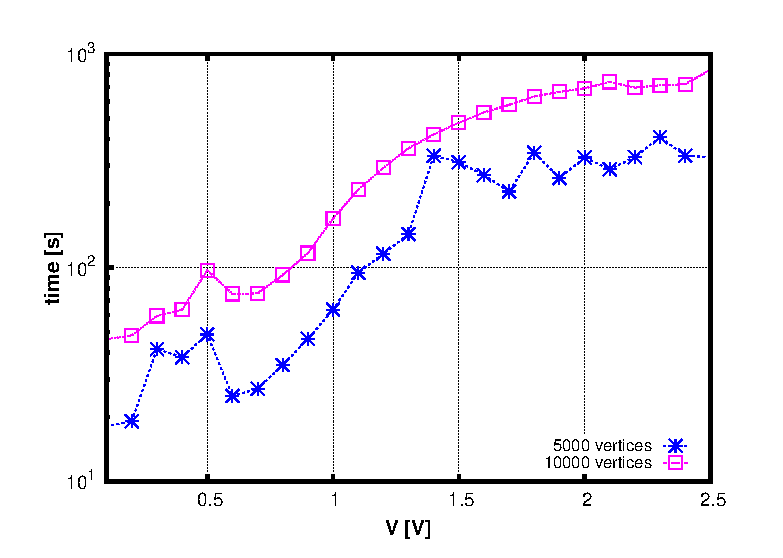
\includegraphics[height=7cm]
{Results/Caratteristiche/Diode/ComputationalTimeDifferentMeshes.eps}
\caption{Total time Gummel Map.}
 \label{fig: tempi computazionali 1}
 \end{figure}
 
 Let us consider the case with a coarse mesh. In \figref{fig: tempi computazionali 2} it is clear how the average time spent to solve the NLP and the DD equations remains almost unchanged. On the contrary the number of GM iterations needed by the system to reach the solution, increases for voltages above $\approx 1.5[V]$.

A possible explanation of this trend can be found comparing solution and initial guess for a bias below and above $1.5[V]$ (similar considerations can be done for carrier densities). When voltage is low, like in \figref{fig: different biast initial step 1} ($V_A = 0.1[V]$), the potential shape is well predicted by the initial guess, resulting in a better convergence for the Gummel map algorithm. On the contrary in \figref{fig: different biast initial step 2} ($V_A=1.6[V]$) the device operates as a resistence and the potential profile is close to a linear function: this implies that the solution is far from the initial guess of equilibrium condition and the algorithm needs more steps.


 
 \begin{figure}[!t]
\centering
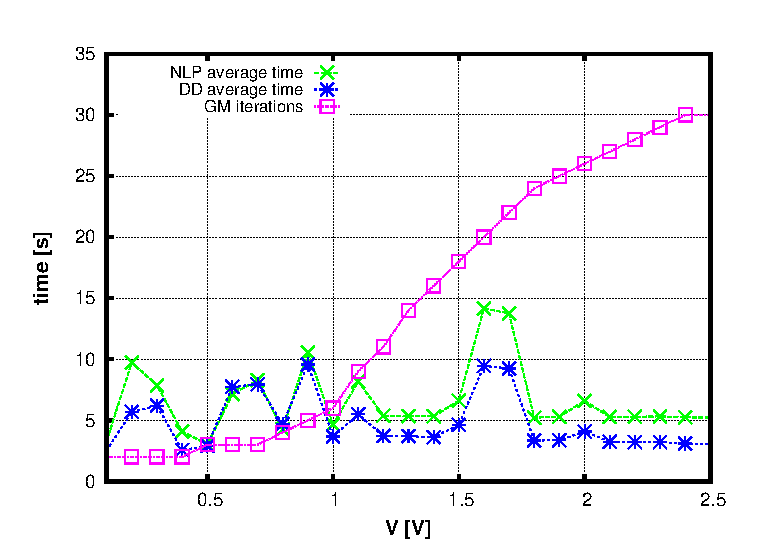
\includegraphics[height=7cm]{Results/Caratteristiche/Diode/ConfrontoTempiNLPDDGMiterations.eps}
\caption{Time to solve the NLP and DD equations, and number of  iterations of the Gummel map.}
\label{fig: tempi computazionali 2}
\end{figure}

\begin{figure}[!b]
\centering
\subfloat[][\label{fig: different biast initial step 1}]
{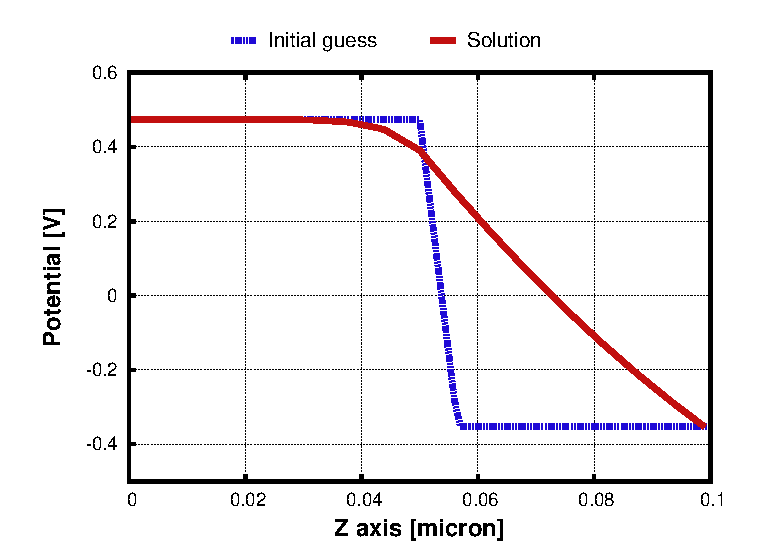
\includegraphics[height=4.5cm]{DatiImmaginiTESI/Diode/PotentialZaxis01volt.eps}}
\subfloat[][\label{fig: different biast initial step 2}]
{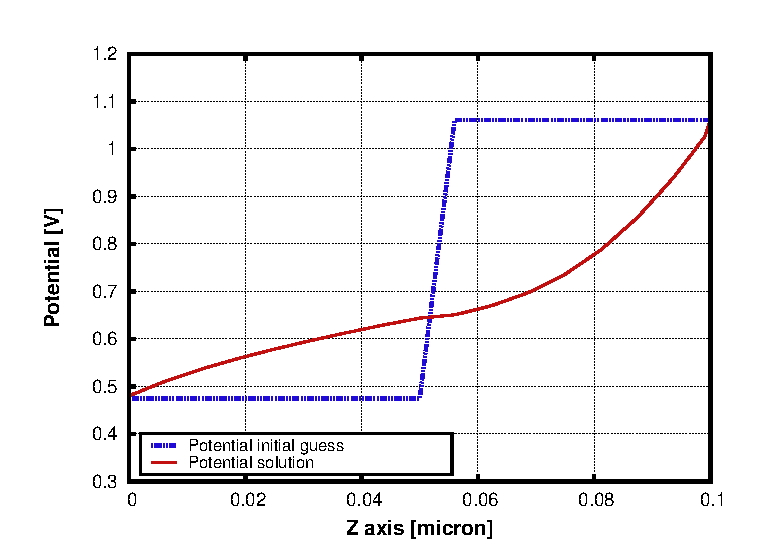
\includegraphics[height=4.5cm]{DatiImmaginiTESI/Diode/PotentialZaxis15volt.eps}}
\caption{Initial guess for different bias compared with the final solution of the device of \figref{fig: diodo struttura}.}
\label{fig: different biast initial step}
\end{figure}
 



\clearpage


\subsection{p-n junction in oxide}
\label{sec: PNOX}

In this test case a silicon p-n junction $0.3[\mu m]$ long is surrounded by an oxide layer $0.025[\mu m]$ thick. The section of the silicon part is a $0.1 \times 0.1 [\mu m^2]$ square.  We employ $6334$ vertices and $33121$ elements overall the domain. The structure and the doping are shown in \figref{fig: structure diodeox}. The setting of the electrodes is similar to the previous test case and contacts are defined only on silicon surface. 
\tabref{tab: diodeox 3d} reports settings, models and parameters used in the simulations.

\figref{fig: plot 1D diodeox} shows the solutions and the quasi Fermi potential levels along a line parallel to the Z-axis and placed at the center of the device. The main features are similar to the previous test case, also for the boundary layers at contact for carriers and quasi Fermi potentials.
\figsref{fig: potential diodeox}-\ref{fig: hdensity diodeox} show the 3D solutions for the test at $0.3[V]$, while \figref{fig: potential diodeox 1V}-\ref{fig: hdensity diodeox 1V} refer to the case at $1.0[V]$. Both the 1D cuts and 3D plots agreement with the commercial software are very good. 

\vspace{0.5cm}

\begin{figure}[!h]
\centering
\subfloat[][\emph{Mesh}]
{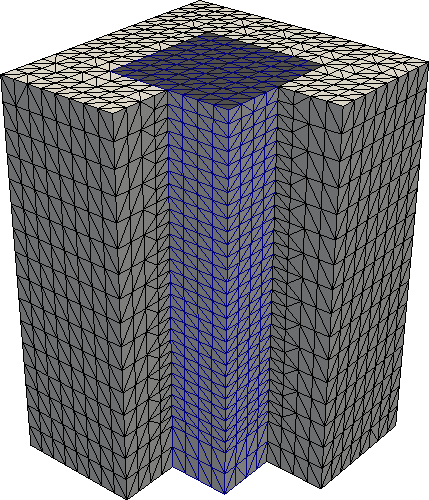
\includegraphics[width=0.33\textwidth , height=5cm]{Results/DIODEOX/AAA_structureandcontact2.png}}
\hspace{0.06\textwidth}
\subfloat[][\emph{Doping concentration}]
{\includegraphics[width=0.33\textwidth ,height=5cm]{Results/DIODEOX/AAA_Dopingconcentration2.png}}
\hspace{0.04\textwidth}
{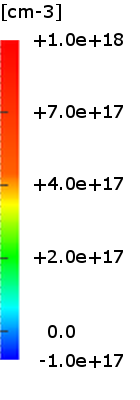
\includegraphics[width=0.1\textwidth ,height=4.5cm]{Results/DIODEOX/LegendDopingDiodeOx.png}}
\caption{Test case p-n junction in oxide.}
\label{fig: structure diodeox}
\end{figure}


\vspace{0.5cm}

\begin{table}[!h]
\centering
\begin{tabular}{ccccc}
\toprule
 Test case  & Mobility model & \multirow{2}*{R/G model} & \multirow{2}*{$\epsilon_{Si}$} & \multirow{2}*{$\epsilon_{0x}$}  \\
 $[V]$ & $[cm^2V^{-1}s^{-1}]$ & & & \\
\midrule
$V_A=0.3$ & $\mu_n = 1417$, $\mu_p = 470.5$ & SRH, Auger & 11.6 & 3.9 \\
$V_A=1.0$ & $\mu_n = 1417$, $\mu_p = 470.5$ & SRH, Auger & 11.6 & 3.9 \\\bottomrule
\end{tabular}
\caption{p-n junction in oxide - list of settings, parameters and models.}
\label{tab: diodeox 3d}
\end{table}




\begin{figure}[!t]
\centering

\subfloat[][\emph{Electrostatic potential.}]
{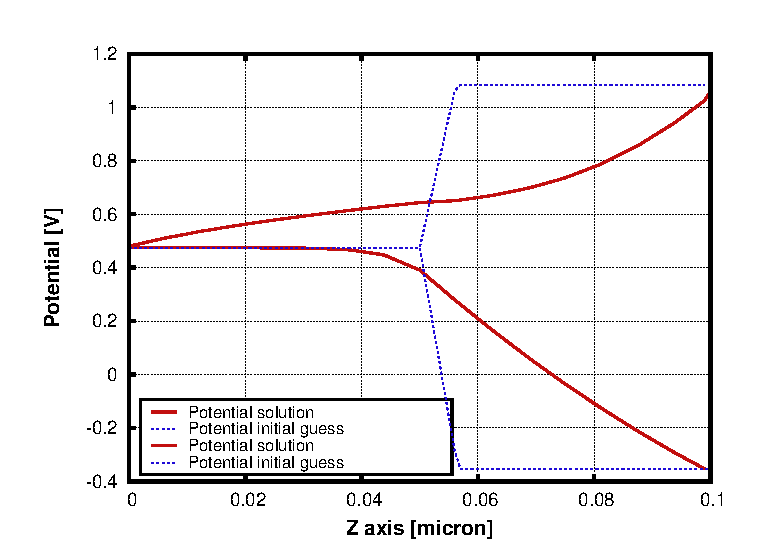
\includegraphics[width=0.5\textwidth , height=5cm]{DatiImmaginiTESI/DiodeOx/PotentialZaxis.eps}}
\subfloat[][\emph{Electrostatic potential.}]
{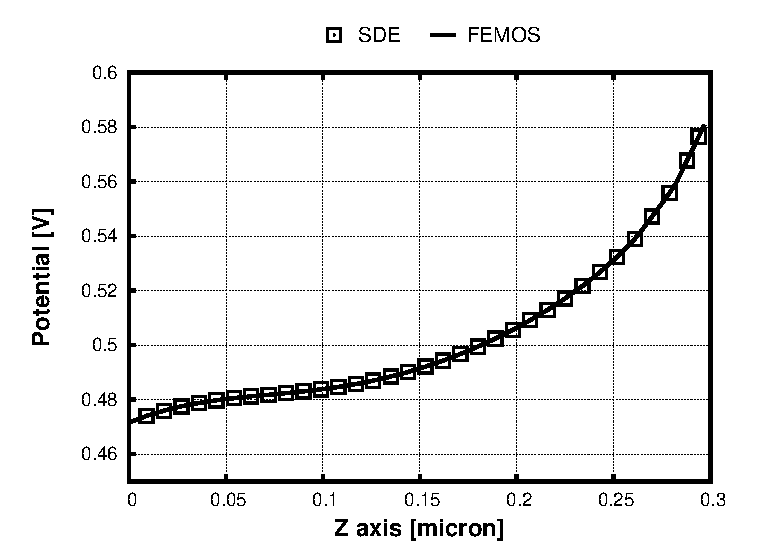
\includegraphics[width=0.5\textwidth , height=5cm]{DatiImmaginiTESI/DiodeOx/PotentialZaxis1VOLT.eps}}


\subfloat[][\emph{Hole and electron densities.}]
{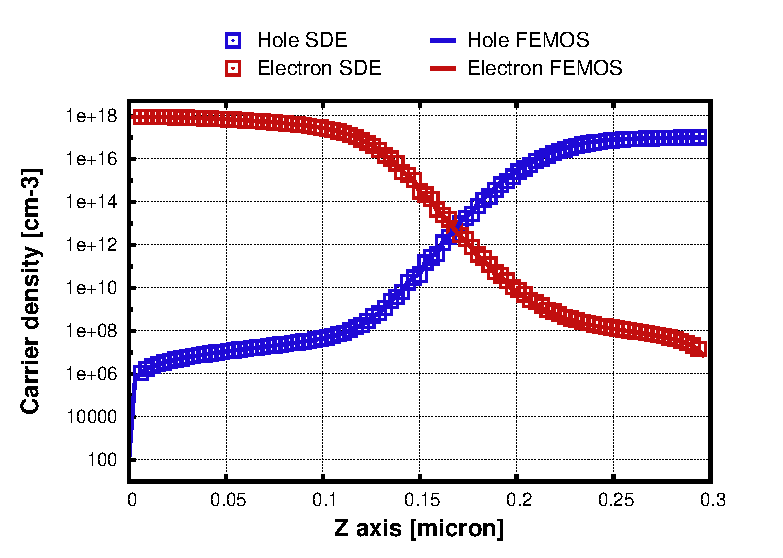
\includegraphics[width=0.5\textwidth , height=5cm]{DatiImmaginiTESI/DiodeOx/DensityZaxis.eps}}
\subfloat[][\emph{Hole and electron densities.}]
{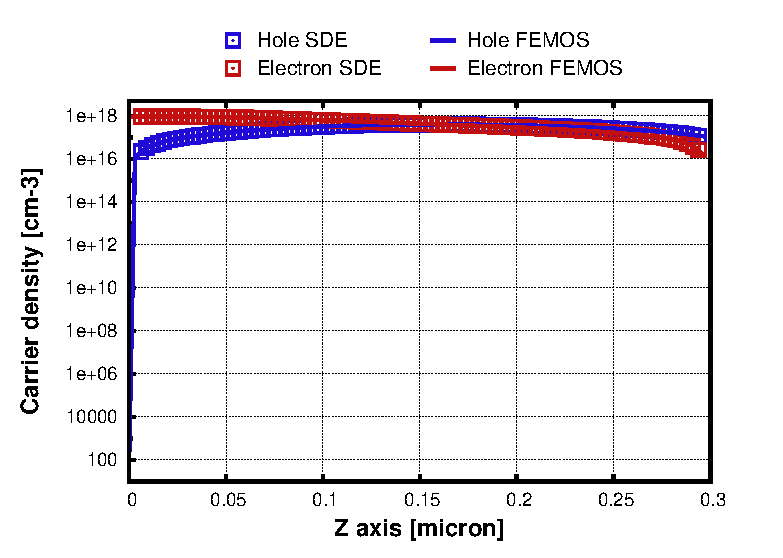
\includegraphics[width=0.5\textwidth , height=5cm]{DatiImmaginiTESI/DiodeOx/DensityZaxis1VOLT.eps}}


\subfloat[][\emph{Quasi Fermi potential levels.}]
{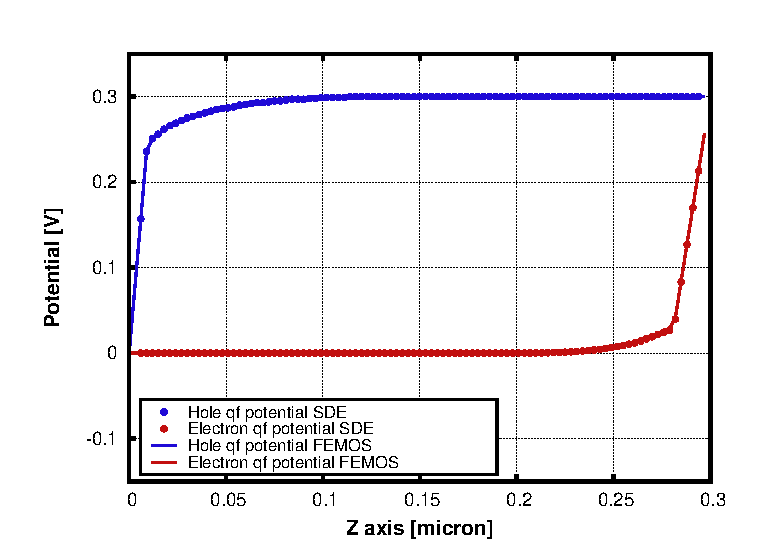
\includegraphics[width=0.5\textwidth , height=5cm]{DatiImmaginiTESI/DiodeOx/QFPotentialZaxis.eps}}
\subfloat[][\emph{Quasi Fermi potential levels.}]
{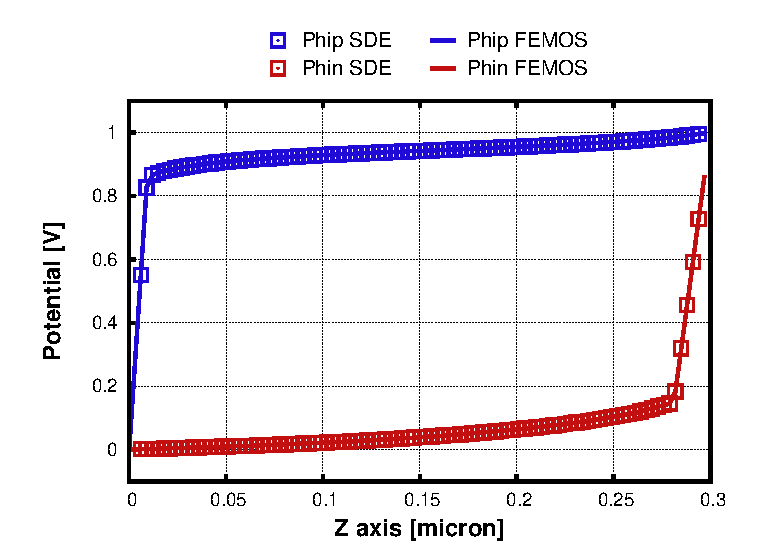
\includegraphics[width=0.5\textwidth , height=5cm]{DatiImmaginiTESI/DiodeOx/QFPotentialZaxis1VOLT.eps}}


\caption{1D plots of the solutions and the quasi Fermi potential levels along the line parallel to the Z-axis and placed at the center of the device of \figref{fig: structure diodeox}. On the left test case at $V_A=0.3[V]$ is reported while on the right at $V_A=1.0[V]$.}
\label{fig: plot 1D diodeox}
\end{figure}

\clearpage


\begin{figure}[!h]
\centering
\subfloat[][\emph{FEMOS}]
{\includegraphics[width=0.3\textwidth ,height=4.5cm]{Results/DIODEOX/FEMOS1817_potential03volt.png}}
\hspace{0.1\textwidth}
\subfloat[][\emph{SDEVICE}]
{\includegraphics[width=0.3\textwidth ,height=4.5cm]{Results/DIODEOX/FEMOS1817_potential03volt.png}}
\hspace{0.04\textwidth}
{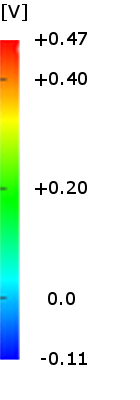
\includegraphics[width=0.1\textwidth ,height=4.5cm]{Results/DIODE/LegendPotentialDiode03volt.png}}
\caption{p-n junction in oxide 0.3[V] - ElectrostaticPotential.}
\label{fig: potential diodeox}
\end{figure}

\vspace{0.5cm}

\begin{figure}[!h]
\centering
\subfloat[][\emph{FEMOS}]
{\includegraphics[width=0.3\textwidth ,height=4.5cm]{Results/DIODEOX/FEMOS1817_edensity03volt.png}}
\hspace{0.1\textwidth}
\subfloat[][\emph{SDEVICE}]
{\includegraphics[width=0.3\textwidth ,height=4.5cm]{Results/DIODEOX/FEMOS1817_edensity03volt.png}}
\hspace{0.04\textwidth}
{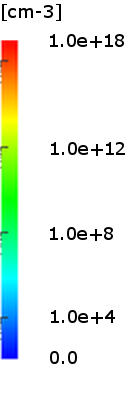
\includegraphics[width=0.1\textwidth ,height=4.5cm]{Results/DIODEOX/LegendEdensityDiodeOx03volt.png}}
\caption{p-n junction in oxide 0.3[V] - Electron density.}
\label{fig: edensity diodeox}
\end{figure}

\vspace{0.5cm}

\begin{figure}[!h]
\centering
\subfloat[][\emph{FEMOS}]
{\includegraphics[width=0.3\textwidth ,height=4.5cm]{Results/DIODEOX/FEMOS1817_hdensity03volt.png}}
\hspace{0.1\textwidth}
\subfloat[][\emph{SDEVICE}]
{\includegraphics[width=0.3\textwidth ,height=4.5cm]{Results/DIODEOX/FEMOS1817_hdensity03volt.png}}
\hspace{0.04\textwidth}
{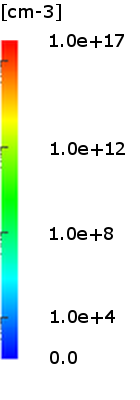
\includegraphics[width=0.1\textwidth ,height=4.5cm]{Results/DIODEOX/LegendHdensityDiodeOx03volt.png}}
\caption{p-n junction in oxide 0.3[V] - Hole density.}
\label{fig: hdensity diodeox}
\end{figure}

\clearpage


\begin{figure}[!h]
\centering
\subfloat[][\emph{FEMOS}]
{\includegraphics[width=0.3\textwidth ,height=4.5cm]{Results/DIODEOX/FEMOS1817_potential1voltONLYDEVICE.png}}
\hspace{0.1\textwidth}
\subfloat[][\emph{SDEVICE}]
{\includegraphics[width=0.3\textwidth ,height=4.5cm]{Results/DIODEOX/FEMOS1817_potential1voltONLYDEVICE.png}}
\hspace{0.04\textwidth}
{\includegraphics[width=0.1\textwidth ,height=4.5cm]{Results/DIODE/LegendPotentialDiode1volt.png}}
\caption{p-n junction in oxide 1.0[V] - Electrostatic Potential.}
\label{fig: potential diodeox 1V}
\end{figure}

\vspace{0.5cm}

\begin{figure}[!h]
\centering
\subfloat[][\emph{FEMOS}]
{\includegraphics[width=0.3\textwidth ,height=4.5cm]{Results/DIODEOX/EdensityLINEARDIODEOXONLYDEVICE.png}}
\hspace{0.1\textwidth}
\subfloat[][\emph{SDEVICE}]
{\includegraphics[width=0.3\textwidth ,height=4.5cm]{Results/DIODEOX/EdensityLINEARDIODEOXONLYDEVICE.png}}
\hspace{0.04\textwidth}
{\includegraphics[width=0.1\textwidth ,height=4.5cm]{Results/DIODEOX/LegendEdensityDiodeOx1volt.png}}
\caption{p-n junction in oxide 1.0[V] - Electron density.}
\label{fig: edensity diodeox 1V}
\end{figure}

\vspace{0.5cm}

\begin{figure}[!h]
\centering
\subfloat[][\emph{FEMOS}]
{\includegraphics[width=0.3\textwidth ,height=4.5cm]{Results/DIODEOX/HdensityLINEARDIODEOXONLYDEVICE.png}}
\hspace{0.1\textwidth}
\subfloat[][\emph{SDEVICE}]
{\includegraphics[width=0.3\textwidth ,height=4.5cm]{Results/DIODEOX/HdensityLINEARDIODEOXONLYDEVICE.png}}
\hspace{0.04\textwidth}
{\includegraphics[width=0.1\textwidth ,height=4.5cm]{Results/DIODEOX/LegendHdensityDiodeOx1volt.png}}
\caption{p-n junction in oxide 1.0[V] - Hole density.}
\label{fig: hdensity diodeox 1V}
\end{figure}

\clearpage





\subsubsection{3D effect on the electric field}


\figref{fig: potential diodeox} shows how, at low bias, the electrostatic potential behaves in a different manner in the oxide with the respect to the silicon region.
Since we impose $\nabla \varphi \cdot \vect{n}=0$ on the oxide boundary no field lines of the electric field can cross that boundary and, as a consequence, field lines can start and end only at contact A or B.
The electric field inside the device is due only to the displacement effect in the junction of the silicon which imposes the electric response also in the oxide material where the solution is no more linear. \figref{fig: electric field diode} reports the electric field lines in the case of $V_A=0.3[V]$ compared with the commercial software: agreement is very good. The lower magnitude of the electric field in the oxide, results in a more diffused potential.

At high bias (\figref{fig: potential diodeox 1V}) the influence of the contacts (A,B) becomes higher and the electrostatic potential is much more similiar in the two subdomains.


\vspace{1cm}

\begin{figure}[!h]
\centering
\subfloat[][\emph{FEMOS}]
{\includegraphics[width=0.38\textwidth ,height=5.5cm]{Results/DIODEOX/FEMOS1817_electricfield03volt.png}}
\hspace{0.05\textwidth}
\subfloat[][\emph{SDEVICE}]
{\includegraphics[width=0.38\textwidth ,height=5.5cm]{Results/DIODEOX/SDEVICE1817_electricfield03volt.png}}
\hspace{0.04\textwidth}
{\includegraphics[width=0.1\textwidth ,height=5cm]{Results/DIODEOX/LegendElectricFieldDiodeOx03volt.png}}
\caption{Test case dide p-n in oxide 0.3[V] - Electric field.}
\label{fig: electric field diode}
\end{figure}

\vspace{0.5cm}


It is important to notice that the displacement formulation approach does not satisfied  in a strong manner the princinple of action and reaction at boundaries.
This is equivalent to saying that given two elements $K_i,K_j\in \mathcal{T}_h$ such that $K_i \bigcap K_j = f_i$ where $f_i \in \mathcal{F}_h$ and denoting by $\vect{n}_{i}$ the outward normal vector of $\partial K_i$ and $\vect{n}_{j}$ the outward normal vector of $\partial K_j$,  the following equations are satisfied only in a weak sense:

\begin{align}
\vect{D}|_{K_i}\cdot \vect{n}_{i} & = \vect{D}|_{K_j} \cdot \vect{n}_{j} \label{eq: conservazione vettore spostamento}\\
\vect{J}_n|_{K_i}\cdot \vect{n}_{i} & = \vect{J}_n|_{K_j}\cdot \vect{n}_{j} \\
\vect{J}_p|_{K_i}\cdot \vect{n}_{i} & = \vect{J}_p|_{K_j}\cdot \vect{n}_{j} .
\end{align}


In fact, taking in consideration equation \referenzaeq{eq: conservazione vettore spostamento}, we can state that along the interface silicon-oxide the following equality holds

\begin{equation}
\label{eq: rapporto campi}
\epsilon_{ox}\vect{E}|_{K_i}\cdot \vect{n}_{i} = \epsilon_{Si}\vect{E}|_{K_j} \cdot \vect{n}_{j} \psp{5} \Rightarrow \psp{5}  [\vect{E}|_{K_i}]_y = \dfrac{\epsilon_{Si}}{\epsilon_{ox}}[\vect{E}|_{K_j}]_y.
\end{equation}  

According with the parameters used in the simulations the jump of the electric field component from oxide to semiconductor is around $3.00$. \figref{fig: salto electric field} shows the plots of $E_y$ along a line parallel to the Y-axis crossing both oxide and silicon: the ratio expressed by \referenzaeq{eq: rapporto campi} is almost $3.6$ at $y=0.05[\mu m]$ and $y = 0.15[\mu m]$ where the interfaces are located.

Each tetrahedral interface of the partition is affected by the same problem, which means that the normal component of the electric field from one element of the grid to the neighbouring is not conserved even if the material is homogeneous and there is no charge at the interface. Despite this drawback, the solutions are acceptable. But if we would like to satisfy equation \referenzaeq{eq: conservazione vettore spostamento} in a strong manner, the use of a mixed-hybrid formulation is needed which ensures the conservation of the flux also under possbile strong discontinuities of material properties.


\begin{figure}[!h]
\centering
\includegraphics[height=5cm]{DatiImmaginiTESI/DiodeOx/ElectricFieldYaxis.eps}
\caption{$E_y$ along a line parallel to Y-axis, $z=0.22[\mu m]$ and $x=0.1[\mu m]$.}
\label{fig: salto electric field}
\end{figure}


\clearpage





\subsection{n-channel MOSFET}
\label{sec: MOS}

The description of the working principle of a MOSFET device can be found in \cite{ModernVLSIdevices}: it is a four-terminal device with the electrodes designated as gate (G), source (S), drain (D) and substrate or bulk (B). The gate electrode is usually made of metal or heavily doped polysilicon and is separated from the substrate by a thin silicon dioxide. The surface region under the gate oxide between source and drain is called \textit{channel} region.
Because the current in a MOSFET is due to carriers of one polarity, the MOSFET is usually referred as a unipolar or majority-carrier device: n-channel (n-MOSFET) and p-channel (p-MOSFET) are considered in the test. A \textit{n-MOSFET} (p-MOSFET) consists of a p-type (n-type) silicon substrate into which two n-regions (p-regions) are designed as source and drain. The n-regions (p-regions) are doped according with a Gaussian profile as in a real implantation process. 
\figref{fig: mos geometry 1} and \figref{fig: mos geometry 2} show the geometry and the doping concentration for the n-MOSFET with a coarse mesh ($2739$ vertices and $12338$ elements). 
We note that the mesh has been refined where the more interesting phenomena occur, i.e., along channel and at drain/source contacts.

If a sufficiently large positive voltage is applied to the gate, the silicon surface is inverted to n-type (p-type), which forms a conducting channel between the source and drain: applying a small positive voltage to the drain (source) the electrons (holes) start to flow from source (drain) to drain (source) and therefore a current is generated. 

\begin{figure}[!b]
\centering
\subfloat[][\emph{Mesh}\label{fig: mos geometry 1}]
{\includegraphics[width=0.38\textwidth ,height=4.3cm]
{Results/MOS/AAA_MeshAndContact.png}}
\hspace{0.06\textwidth}
\subfloat[][\emph{Doping concentration}\label{fig: mos geometry 2}]
{\includegraphics[width=0.38\textwidth ,height=4.3cm]{Results/MOS/AAA_DopingConcentration.png}}
{\includegraphics[width=0.1\textwidth ,height=4.5cm]{Results/MOS/LegendDopingNMOS.png}}
\caption{Geometry of a n-channel MOSFET.}
\label{fig: mos geometry}
\end{figure}




The visualization of the MOSFET working principle is better clarified in \figref{fig: energy levels MOS} where the band profile along the channel axis is reported for two different gate bias.
The voltage applied to the gate tends to decrease the energy barrier in the channel region: a little drain voltage causes the flow of the electrons.
\figref{fig: channel figures 1D} shows the profile of carrier concentrations in the middle of the channel with a cut perpendicular to the gate, for off-state and on-state: the inversion occurs when the gate voltage is higher than the well known threshold voltage.
\figref{fig: channel figures 3D} shows the 3D view of the n-channel space charge after inversion.



\begin{figure}[!t]
\centering
\subfloat[][\emph{$V_G=0.0[V]$, $V_D=0.1[V]$}]
{\includegraphics[width=0.5\textwidth , height = 5cm]{DatiImmaginiTESI/Mos/BandDiagramMOS0volt.eps}}
\subfloat[][\emph{$V_G=2.0[V]$, $V_D=0.1[V]$}]
{\includegraphics[width=0.5\textwidth , height = 5cm]{DatiImmaginiTESI/Mos/BandDiagramMOS2volt.eps}}
\caption{Energy band levels for a n-MOSFET along the channel.}
\label{fig: energy levels MOS}
\end{figure}

Finally \figref{fig: electric field mos} reports the streamline plot of the electric field inside the device for FEMOS and the SDEVICE in the case of on-state MOSFET.


Settings, parameters and models used for these simulations are summarized in \tabref{tab: mos direct pol}. \figsref{fig: potential mos off}-\ref{fig: pdensity mos off} show the 3D view of the electrostatic potential, electron and hole densities obtained by FEMOS and by the commercial code in the off-state ($V_G=0.0[V]$), while \figsref{fig: potential mos}-\ref{fig: pdensity mos} refer to the on-state ($V_G=2.0[V]$): the agreement is very good.



\begin{table}[!h]
\centering
\begin{tabular}{ccccc}
\toprule
 Test case  & Mobility model  & \multirow{2}*{R/G model} & \multirow{2}*{$\epsilon_{Si}$} & \multirow{2}*{$\epsilon_{0x}$}  \\
 $[V]$ & $[cm^2V{-1}s^{-1}]$ & & & \\
\midrule
 $V_G=0.0 [V]$, $V_D=0.0[V]$,& $\mu_n = 1417$ & \multirow{2}*{SRH, Auger, II} & \multirow{2}*{11.6} & \multirow{2}*{3.9} \\
 $V_S=V_B=0.0[V]$ & $\mu_p = 470.5$ & & & \\ 
\midrule
$V_G=2.0 [V]$, $V_D=0.1[V]$,& $\mu_n = 1417$ & \multirow{2}*{SRH, Auger} & \multirow{2}*{11.6} & \multirow{2}*{3.9} \\
 $V_S=V_B=0.0[V]$ & $\mu_p = 470.5$ & & & \\
 \bottomrule
\end{tabular}
\caption{n-MOSFET - list of settings, parameters and models.}
\label{tab: mos direct pol}
\end{table}




\begin{figure}[!h]
\centering
\subfloat[][1D cut perpendicular to the channel. \label{fig: channel figures 1D}]
{\includegraphics[width=0.5\textwidth ,height=5cm]{DatiImmaginiTESI/Mos/DensityZaxis.eps}}
\hspace{0.02\textwidth}
\subfloat[][Space charge.\label{fig: channel figures 3D}]
{\includegraphics[width=0.3\textwidth ,height=4.5cm]{Results/PlotOverLine/Mos/Contour3DSpacechargeONLYDEVICE}}
\hspace{0.04\textwidth}
{\includegraphics[width=0.1\textwidth ,height=4.5cm]{Results/MOS/LegendSpaceChargeNMOS.png}}
\caption{Channel of the n-MOSFET.}
\label{fig: channel figures}
\end{figure}

\vspace{0.5cm}

\begin{figure}[!h]
\centering
\subfloat[][\emph{FEMOS}]
{\includegraphics[width=0.38\textwidth ,height=4.5cm]{Results/MOS/MOSelectricfield.png}}
%FEMOS181718_ElectricField2voltONLYDEVICE.png}}
\hspace{0.06\textwidth}
\subfloat[][\emph{SDEVICE}]
{\includegraphics[width=0.38\textwidth ,height=4.5cm]{Results/MOS/SDEVICE181718_ElectricField2voltONLYDEVICE.png}}
\hspace{0.04\textwidth}
{\includegraphics[width=0.1\textwidth ,height=4.5cm]{Results/MOS/LegendElectricFieldNMOS.png}}
\caption{n-MOSFET $V_G = 2.0 [V]$ - Electric field.}
\label{fig: electric field mos}
\end{figure}



\clearpage

\begin{figure}[!h]
\centering
\subfloat[][\emph{FEMOS}]
{\includegraphics[width=0.38\textwidth ,height=4.5cm]{Results/MOS/MOSNelectrostaticpotSUBTHRESONLYDEVICE.png}}
\hspace{0.06\textwidth}
\subfloat[][\emph{SDEVICE}]
{\includegraphics[width=0.38\textwidth ,height=4.5cm]{Results/MOS/MOSNelectrostaticpotSUBTHRESONLYDEVICE.png}}
\hspace{0.04\textwidth}
{\includegraphics[width=0.1\textwidth ,height=4.5cm]{Results/MOS/LegendPotentialNMOSdirect.png}}
\caption{n-MOSFET $V_G = 0.0 [V]$ - Electrostatic potential.}
\label{fig: potential mos off}
\end{figure}

\vspace{0.5cm}

\begin{figure}[!h]
\centering
\subfloat[][\emph{FEMOS}]
{\includegraphics[width=0.38\textwidth ,height=4.5cm]{Results/MOS/MOSNedensitySUBTHRESONLYDEVICE.png}}
\hspace{0.06\textwidth}
\subfloat[][\emph{SDEVICE}]
{\includegraphics[width=0.38\textwidth ,height=4.5cm]{Results/MOS/MOSNedensitySUBTHRESONLYDEVICE.png}}
\hspace{0.04\textwidth}
{\includegraphics[width=0.1\textwidth ,height=4.5cm]{Results/MOS/LegendEdensityNMOSdirect.png}}
\caption{n-MOSFET $V_G = 0.0 [V]$ - Electron density.}
\label{fig: ndensity mos off}
\end{figure}

\vspace{0.5cm}

\begin{figure}[!h]
\centering
\subfloat[][\emph{FEMOS}]
{\includegraphics[width=0.38\textwidth ,height=4.5cm]{Results/MOS/MOSNhdensitySUBTHRESONLYDEVICE.png}}
\hspace{0.06\textwidth}
\subfloat[][\emph{SDEVICE}]
{\includegraphics[width=0.38\textwidth ,height=4.5cm]{Results/MOS/MOSNhdensitySUBTHRESONLYDEVICE.png}}
\hspace{0.04\textwidth}
{\includegraphics[width=0.1\textwidth ,height=4.5cm]{Results/MOS/LegendHdensityNMOSdirect.png}}
\caption{n-MOSFET $V_G = 0.0 [V]$ - Hole density.}
\label{fig: pdensity mos off}
\end{figure}






\clearpage

\begin{figure}[!h]
\centering
\subfloat[][\emph{FEMOS}]
{\includegraphics[width=0.38\textwidth ,height=4.5cm]{Results/MOS/FEMOS181718_potential2voltONLYDEVICE.png}}
\hspace{0.06\textwidth}
\subfloat[][\emph{SDEVICE}]
{\includegraphics[width=0.38\textwidth ,height=4.5cm]{Results/MOS/FEMOS181718_potential2voltONLYDEVICE.png}}
\hspace{0.04\textwidth}
{\includegraphics[width=0.1\textwidth ,height=4.5cm]{Results/MOS/LegendPotentialNMOSdirectON.png}}
\caption{n-MOSFET $V_G = 2.0 [V]$ - Electrostatic potential.}
\label{fig: potential mos}
\end{figure}

\vspace{0.5cm}

\begin{figure}[!h]
\centering
\subfloat[][\emph{FEMOS}]
{\includegraphics[width=0.38\textwidth ,height=4.5cm]{Results/MOS/FEMOS181718_ndensity2voltONLYDEVICE.png}}
\hspace{0.06\textwidth}
\subfloat[][\emph{SDEVICE}]
{\includegraphics[width=0.38\textwidth ,height=4.5cm]{Results/MOS/FEMOS181718_ndensity2voltONLYDEVICE.png}}
\hspace{0.04\textwidth}
{\includegraphics[width=0.1\textwidth ,height=4.5cm]{Results/MOS/LegendEdensityNMOSdirectON.png}}
\caption{n-MOSFET $V_G = 2.0 [V]$ - Electron density.}
\label{fig: ndensity mos}
\end{figure}

\vspace{0.5cm}

\begin{figure}[!h]
\centering
\subfloat[][\emph{FEMOS}]
{\includegraphics[width=0.38\textwidth ,height=4.5cm]{Results/MOS/FEMOS181718_pdensity2volt.png}}
\hspace{0.06\textwidth}
\subfloat[][\emph{SDEVICE}]
{\includegraphics[width=0.38\textwidth ,height=4.5cm]{Results/MOS/FEMOS181718_pdensity2volt.png}}
\hspace{0.04\textwidth}
{\includegraphics[width=0.1\textwidth ,height=4.5cm]{Results/MOS/LegendHdensityNMOSdirect.png}}
\caption{n-MOSFET $V_G = 2.0 [V]$ - Hole density.}
\label{fig: pdensity mos}
\end{figure}




\subsubsection{Reverse bias}
\label{sec: inv pol mos}

In Section \ref{sec: continuity equations} we pointed out that the discretization scheme (EAFE) cannot satisfy the discrete maximum principle in 3D simulations unless we satisfy condition  \referenzaeq{eq: mesh delaunay condition}.  Therefore it is possible to encounter situations where negative solutions are obtained and this usually happens when the concentration of electrons and holes become low.

In order to highlight this possible critical situation, a n-channel MOSFET is simulated in reverse bias regime by grounding all the contacts except the drain which is ramped to $0.5[V]$: \tabref{tab: nmos inverse} reports the needed indications for the simulation.

\figref{fig: negative carriers MOS} reports the electron density computed with FEMOS and SDEVICE using the mesh presented in \figref{fig: mos geometry 2}: the results are comparable, but near the drain-bulk junction FEMOS presents some points with negative concentrations. Increasing drain bias the phenomenon tends to spread over a larger area, until it affects irremediably the simulation of the device.
As we anticipated in Chapter \ref{chap: finite element}, the most practice technique to limit this problem is local mesh refinement.
\figref{fig: drain stress mos 13000 1} represents a finer mesh with $13000$ points and $67388$ elements. Using this mesh the correctness of the solution is recovered \figref{fig: drain stress mos 13000 2}. \figref{fig: zikatanov mos} shows how the satisfaction of \referenzaeq{eq: mesh delaunay condition} changes between the different meshes: increasing the number of vertices over the critical region a better fulfillment of \referenzaeq{eq: mesh delaunay condition} is guaranteed. 
Results suggest that in order to treat this situation it may be useful to implement a suitable a-posteriori error estimation and adaptive mesh refinement techniques. 

Finally \figref{fig: pot MOS negative} and \figref{fig: hole MOS negative} report FEMOS electrostatic potential and hole density for the finer mesh compared with the commercial tool: the agreement is very good.

\begin{table}[!h]
\centering
\begin{tabular}{ccccc}
\toprule
 Test case  & Mobility model  & \multirow{2}*{R/G model} & \multirow{2}*{$\epsilon_{Si}$} & \multirow{2}*{$\epsilon_{0x}$}  \\
 $[V]$ & $[cm^2V{-1}s^{-1}]$ & & & \\
\midrule
 $V_G=0.0$, $V_D=0.5$,& $\mu_n = 1417$ & \multirow{2}*{SRH, Auger, II} & \multirow{2}*{11.6} & \multirow{2}*{3.9} \\
 $V_S=V_B=0.0$ & $\mu_p = 470.5$ & & & \\ 
 \bottomrule
\end{tabular}
\caption{n-MOSFET (reverse bias) - list of settings, parameters and models.}
\label{tab: nmos inverse}
\end{table}



\clearpage 



\begin{figure}[!h]
\centering
\subfloat[][\emph{FEMOS}]
{\includegraphics[width=0.38\textwidth ,height=4.5cm]{Results/Drainstress/NegativeCarrierOnlydevice.png}}
\hspace{0.06\textwidth}
\subfloat[][\emph{SDEVICE}]
{\includegraphics[width=0.38\textwidth ,height=4.5cm]{Results/Drainstress/CarrierSDEonlydevice.png}}
\hspace{0.04\textwidth}
{\includegraphics[width=0.1\textwidth ,height=4.5cm]{Results/Drainstress/LegendEdensityNMOSinverse.png}}
\caption{n-MOSFET reverse bias: negative carriers spots for the electron density solution.}
\label{fig: negative carriers MOS}
\end{figure}

\begin{figure}[!h]
\centering
\subfloat[][\emph{Mesh} \label{fig: drain stress mos 13000 1}]
{\includegraphics[width=0.38\textwidth ,height=4.5cm]{Results/Drainstress/MosMeshFitted.png}}
\hspace{0.06\textwidth}
\subfloat[][\emph{FEMOS} \label{fig: drain stress mos 13000 2}]
{\includegraphics[width=0.38\textwidth ,height=4.5cm]{Results/Drainstress/NegativeCarrier13000onlydevice.png}}
\hspace{0.04\textwidth}
{\includegraphics[width=0.1\textwidth ,height=4.5cm]{Results/Drainstress/LegendEdensityNMOSinverse.png}}
\caption{n-MOSFET reverse bias: electron density with finer mesh.}
\label{fig: drain stress mos 13000}
\end{figure}

\begin{figure}[!h]
\centering
\subfloat[][\emph{Coarse mesh.}]
{\includegraphics[width=0.38\textwidth ,height=4.5cm]{Results/Drainstress/Zikatanov3000.png}}
\hspace{0.06\textwidth}
\subfloat[][\emph{Fine mesh.}]
{\includegraphics[width=0.38\textwidth ,height=4.5cm]{Results/Drainstress/Zikatanov13000.png}}
\hspace{0.04\textwidth}
{\includegraphics[width=0.1\textwidth ,height=4.5cm]{Results/Drainstress/LegendZikatanov.png}}
\caption{n-MOSFET: Zikatanov condition.}
\label{fig: zikatanov mos}
\end{figure}

\clearpage

\begin{figure}[!h]
\centering

\subfloat[][\emph{FEMOS}]
{\includegraphics[width=0.38\textwidth ,height=4.5cm]{Results/Drainstress/MOSNelectrostaticpotDRAINSTRESSONLYDEVICE.png}}
\hspace{0.06\textwidth}
\subfloat[][\emph{SDEVICE}]
{\includegraphics[width=0.38\textwidth ,height=4.5cm]{Results/Drainstress/MOSNelectrostaticpotDRAINSTRESSONLYDEVICE.png}}
\hspace{0.04\textwidth}
{\includegraphics[width=0.1\textwidth ,height=4.5cm]{Results/Drainstress/LegendPotentialNMOSinverse.png}}
\caption{n-MOSFET reverse bias - Electrostatic potential.}
\label{fig: pot MOS negative}
\end{figure}


\begin{figure}[!h]

\subfloat[][\emph{FEMOS}]
{\includegraphics[width=0.38\textwidth ,height=4.5cm]{Results/Drainstress/MOSNhdensityDRAINSTRESSONLYDEVICE.png}}
\hspace{1cm}
\subfloat[][\emph{SDEVICE}]
{\includegraphics[width=0.38\textwidth ,height=4.5cm]{Results/Drainstress/MOSNhdensityDRAINSTRESSONLYDEVICE.png}}
\hspace{0.04\textwidth}
{\includegraphics[width=0.1\textwidth ,height=4.5cm]{Results/Drainstress/LegendHdensityNMOSinverse.png}}
\caption{n-MOSFET reverse bias - Hole density.}
\label{fig: hole MOS negative}
\end{figure}

\clearpage

\section{Current evaluation at the Ohmic contacts}

During the analysis of an electric device, one of the most important information is the electrical response at terminals. In order to accomplish this target we have to compute the integral of the electron and hole current density over a generic 2D electrode. We refer here to the procedure found in \cite{ContactCurrentRM} (\textit{residual method}) for the 2D case: the analysis is easily extendable to the 3D case if we consider also \cite{GalerkMethConsHughes}. Moreover we remark that the method can be successfully applied to a wide spread of applications, including contact charges, carrier quantum probability fluxes and heat fluxes.

A contact is defined by a surface: we can consider $\Gamma_{D,Si} = \bigcup_{c=1}^d \Gamma_c$ where $d$ is the number of terminals on the device and $\forall c=1,...,d$, $\Gamma_c$ is the $c$-th contact. For each contact we need to compute the total current $\mathcal{I}_c$ as:

\begin{equation}
\mathcal{I}_c = \mathcal{I}_c^n + \mathcal{I}_c^p
\end{equation}
where $\mathcal{I}_c^n$ and $\mathcal{I}_c^p$ are the contribution of the electron and hole current.
For a given contact $\Gamma_c$, the flux of the current density is defined as

\begin{equation}
\label{eq: current flux}
\mathcal{I}_c^\nu = \int_{\Gamma_c}\vect{J}_\nu(\nu) \cdot \vect{n} \, d{\Gamma} \psp{10} \nu = \{n,p\}
\end{equation}
where $\vect{n}$ is the unit outward normal of the domain boundary. It is well known that the evaluation of boundary integrals is a difficult task. Most problems in \referenzaeq{eq: current flux} arise from singularities in spatial derivatives of the approximate solution $n_h$ or $p_h$ near the contact edges, due to a change in the boundary condition type from Dirichlet to Neumann.

Let $\eta$ be the set of all vertices of the partition $\mathcal{T}_h$ for the discretized electron continuity problem \referenzaeq{eq: weak formulation displacement}. We can split the set of total nodes in contact nodes $\eta_g \in \Gamma_{D,Si}$ and the complementary part $\eta_n \in \Gamma_{N,Si}$. We define an \textit{auxiliary flux} $H_h$ on $\Gamma_{D,Si}$ as

\begin{equation}
H_h = \sum_{i\in\eta_g} H_{h,i} \psi_i .
\end{equation}


Now, given the spaces:

\begin{align*}
\mathcal{V}_h & =  {\rm span}\{\psi_i\}_{i \in \eta_n} \\
\vect{V}_h & =  {\rm span}\{\psi_i\}_{i \in \eta_g}  \\
\mathcal{S}_h & =  \{u \in \mathcal{V}_h \oplus \vect{V}_h: u|_{\Gamma_{D,Si}} = n_D \}
\end{align*}

it is possible to write a modified form of Galerkin method which reads as:

find $n_h  \in \mathcal{S}_h$ and $H_h \in \vect{V}_h$ such that

\begin{equation}
\label{eq: modified galerkin}
(W_h,H_h)_{\Gamma_{D,Si}} = a(W_h,n_h)-F(W_h) \psp{10} \forall W_h \in \mathcal{V}_h \oplus \vect{V}_h
\end{equation}

where $a(\cdot,\cdot)$ is the bilinear form \referenzaeq{eq: weak formulation displacement} and $F(\cdot)$ the associated linear functional.
Equation \referenzaeq{eq: modified galerkin} splits into two subproblems:

\begin{align}
0  & = a(w_h,n_h)-F(w_h) \psp{10} \forall w_h \in \mathcal{V}_h \label{eq: usual problem}\\
(W_h,H_h)_{\Gamma_{D,Si}} & = a(W_h,n_h)-F(W_h) \psp{10} \forall W_h \in \vect{V}_h . \label{eq: flux problem}
\end{align}

Problem \referenzaeq{eq: usual problem} is identical to the unmodified case and can be treated as before or using a different discretization scheme. Once obtained the solution $n_h$, problem \referenzaeq{eq: flux problem} is fully decoupled from \referenzaeq{eq: usual problem} and we can determine $H_h$ as follows

\begin{equation}
\label{eq: flux problem complete}
(H_h,\psi_i)_{\Gamma_{D,Si}} = a(\psi_i,n_h)-F(\psi_i) \psp{10} \forall i \in \eta_g .
\end{equation} 


In \cite{GalerkMethConsHughes}, it is shown that $H_h$ defines the conserved total flux along $\Gamma_{D,Si}$ and according with the boundary condition, the following equality is obtained

\begin{equation}
\label{eq: conservative flux}
\int_{\Gamma_{D,Si}} H_h \, d\Gamma = - \int_{\Omega_{Si}} qR \, d \Omega.
\end{equation}


On the other hand if we apply the divergence theorem to \referenzaeq{eq: LEC system} we get

\begin{equation}
\label{eq: lec divergence theor}
\int_{\Gamma_{D,Si}} \vect{J}_n \cdot \vect{n} \, d\Gamma = \int_{\Omega} - qR \, d\Omega.
\end{equation}

Equations \referenzaeq{eq: conservative flux} and \referenzaeq{eq: lec divergence theor}  lead us to conclude that for all contacts it holds

\begin{equation}
\label{eq: flux current formula}
\mathcal{I}_c^n = \int_{\Gamma_c} H_h \, d\Gamma.
\end{equation}

In order to compute \referenzaeq{eq: flux current formula}, let $\eta_{c}$ be the set of nodes of the contact $\Gamma_c$. Then, the following equalities hold

\begin{equation}
\label{eq: equalities integrals}
\sum_{l \in \eta_c} \int_{\Gamma_c} H_h \psi_l \, d\Gamma 
=  \int_{\Gamma_c} H_h \sum_{l \in \eta_{c}} \psi_l \,d\Gamma 
= \int_{\Gamma_c} H_h \, d\Gamma.
\end{equation}


According with  \referenzaeq{eq: equalities integrals} we can interpret $(H_h,\psi_i)_{\Gamma_{D,Si}}$ as the contribution to the flux at node $i$ and therefore the current at contact $c$ is given by summing this quantity  over the vertices $\eta_{c}$.

The residual method is thus defined as:
given the system matrix $A$ of the Drift-Diffusion equation, the solution $n_h$ and the right hand side $\vect{b}$, the contribution to the total contact current $\forall c = 1,...,d$ is

\begin{equation}
\mathcal{I}_c^n = (An_h-\vect{b})\cdot \mathbb{I}_c
\end{equation} 

where

\begin{equation}
[\mathbb{I}_c]_i := \left\{ \begin{array}{ll}
0 & i \notin \eta_c \\
1 & i \in \eta_c .
\end{array}  \right.
\end{equation} 

These results holds also for the hole continuity equation. 

%Let be $A$ the system matrix of the continuity equation \referenzaeq{eq: matrice continuità} and $\vect{b}$ the relative right hand side before applying boundary conditions.  The linear problem looks as:
%
%\begin{equation}
%\label{eq: discretization before bc}
%\sum_{j\in\eta} A_{ij} \nu_j = b_i \psp{10} \forall i \in \eta
%\end{equation}
%
%
%Notice that the values of $\nu_j$ are known on the contacts and \referenzaeq{eq: discretization before bc} can be rewritten as follows:
%
%\begin{equation}
%\label{eq: discretization before bc 2}
%\begin{cases}
%
%\sum_{j\in\eta_n} A_{ij} \nu_j = b_i - \sum_{j\in\eta_g} A_{ij} \nu_j & \forall i \in \eta_n \\
%\\
%\sum_{j\in\eta_n} A_{ij} \nu_j = b_i - \sum_{j\in\eta_g} A_{ij} \nu_j & \forall i \in \eta_g \\
%
%\end{cases}
%\end{equation}
%
%The first set of equations is the usual linear system which we solve, while the second can be used for boundary flux estimation. 
% Now we define a new test function $v^h_i$ as:
%
%\begin{equation}
%\label{eq: new test function}
%v^h_i=\sum_{j\in\eta_{gi} }\psi_j
%\end{equation}
%
%where $\eta_{gi}$ is the set of nodes lying on $\Gamma_i$. Substituting \referenzaeq{eq: new test function} in \referenzaeq{eq: current flux} we can state that:
%
%\begin{multline}
%\mathcal{I}_i^\nu 
%= \int_{\Gamma_i}\vect{J}_\nu(\nu) \cdot \vect{n} \, d{\Gamma_i}
%= \sum_{j=1}^{n_d}\int_{\Gamma_j}\vect{J}_\nu(\nu) \cdot \vect{n} \,v_i^h \, d{\Gamma_j} \\
%=\sum_{i\in\eta_{gi}}\sum_{j=1}^{n_d}\int_{\Gamma_j}\vect{J}_\nu(\nu) \cdot \vect{n} \, \psi_i \, d{\Gamma_j} 
%= \sum_{i\in \eta_{gi}}\int_{\partial \Omega}\vect{J}_\nu(\nu) \cdot \vect{n} \, \psi_i \, d{\partial \Omega} \\
%= \sum_{i\in \eta_{gi}} \left[ \int_{\Omega}\nabla \cdot \vect{J}_\nu(\nu) \psi_i \, d{\Omega} + \int_{\Omega}\vect{J}_\nu(\nu) \cdot \nabla\psi_i \, d{\Omega} \right] \\
%= \sum_{m\in \eta_{gi}} \left[ \sum_{j\in\eta} A_{ij} \nu_j - b_i  \right] \\
%\end{multline}
%
%The current at contact $i$ is performed by summing the residuals of the matrix $A$.
%
%Per questo è detto metodo dei residui ...
%
%Nel seguito mostriamo alcuni risultati ...
%\clearpage

\subsection{Simulation results}

The residual method is applied to the already analysed devices and compared with the SDEVICE results. In this section, different mobility and recombination/generation models are tested and verified along with the commercial code results.

\subsubsection{p-n junction}

Considering the p-n junction of Section \ref{sec: PN} we ground the B contact and then A contact is ramped from $-7.5[V]$ to $2.0[V]$ in order to obtain the well known diode characteristic. 
\tabref{tab: caratt diodo} reports the parameters used in the simulation.
In  \figref{fig: caratteristica diode} we plot the electron and hole current at contact A.
Diode breakdown voltage is appearing around $-7.0[V]$ and it is quite well aligned with SDEVICE.

\vspace{0.5cm}

\begin{figure}[!h]
\centering
\includegraphics[width = 0.8\textwidth , height=8cm]{Results/Caratteristiche/Diode/CaratteristicaDiode.eps}
\caption{p-n junction characteristic.}
\label{fig: caratteristica diode}
\end{figure}

\vspace{0.5cm}

\begin{table}[!h]
\centering
\begin{tabular}{cccc}
\toprule
 Test case & Mobility model & \multirow{2}*{R/G model} & \multirow{2}*{$\epsilon_{Si}$}\\
 $[V]$  & $[cm^2V^{-1}s^{-1}]$ & & \\
\midrule
$V_A=-7.5 \div 1.5$, & $\mu_n = 1417$& SRH & \multirow{2}*{11.6}\\
 $V_B=0.0$ & $\mu_p = 470.5$ & II, Auger   & \\
 \bottomrule
\end{tabular}
\caption{p-n junction (characteristic) - list of settings, parameters and models.}
\label{tab: caratt diodo}
\end{table}


\figref{fig: SRH Auger RG} shows the different behaviour of the SRH and Auger R/G contribution at two voltages (plots are made along a line parallel to the Z-axis and placed at the center of the device). Under the built-in condition, both SRH and Auger mechanisms are not significant. Auger contribution decreases in the depletion region due to its strict dependence on the carrier concentrations. At the built-in condition the R/G phenomenon quite increase and are distributed over the entire device causing its saturation. The agreement with the commercial tool is very good.

\vspace{0.5cm}

\begin{figure}[!h]
\centering

\subfloat[][\emph{$V_A=0.3[V]$.}\label{fig: RG 0.3 volt}]
{\includegraphics[width=0.48\textwidth , height = 5.3cm]{DatiImmaginiTESI/Diode/SRHZaxis03volt.eps}}
\hspace{0.02\textwidth}
\subfloat[][\emph{$V_A=1.0[V]$.}\label{fig: RG 1 volt}]
{\includegraphics[width=0.48\textwidth , height = 5.3cm]{DatiImmaginiTESI/Diode/SRHZaxis1volt.eps}}

\caption{p-n junction SRH and Auger RG contribution.}
\label{fig: SRH Auger RG}
\end{figure}

\vspace{0.5cm}

\subsubsection{p-n junction in oxide}

For diode in oxide we analyze the influence of the Masetti mobility model introduced in Section \ref{sec: Masetti model}. \figref{fig: diode ox const} reports electron and hole currents at contact A using the constant mobility model, while \figref{fig: diode ox masetti} refers to the Masetti mobility model. 
This model predicts a decreased value of current flow due to the scattering with impurity dopants, as shown in the 1D plot proposed by \figref{fig: diode ox masetti focus}. Agreement with SDEVICE is very good.

\vspace{1cm}

\begin{table}[!h]
\centering
\begin{tabular}{ccccc}
\toprule
 Test case $[V]$ & Mobility model $[cm^2V{-1}s^{-1}]$ & R/G model & $\epsilon_{Si}$ & $\epsilon_{0x}$  \\
\midrule
$V_A=0.0 \div 1.5$, & $\mu_n = 1417$ & SRH & \multirow{2}*{11.6} & \multirow{2}*{3.9} \\
 $V_B=0.0$ & $\mu_p = 470.5$ & II, Auger  & & \\
\midrule
$V_A=0.0 \div 1.5$, & \multirow{2}*{Masetti} & SRH & \multirow{2}*{11.6} & \multirow{2}*{3.9} \\
 $V_B=0.0$ & & II, Auger  & & \\
 \bottomrule
\end{tabular}
\caption{p-n junction in oxide - list of settings, parameters and models.}
\label{tab: par diodeox curr}
\end{table}


\begin{figure}[!h]
\centering
\subfloat[][Constant mobility. \label{fig: diode ox const}]
{\includegraphics[width=0.49\textwidth , height = 5.4cm]{Results/Caratteristiche/DiodeOx/CurrentDiodeOxide.eps}}
\subfloat[][Masetti mobility. \label{fig: diode ox masetti}]
{\includegraphics[width=0.49\textwidth ,height = 5.4cm]{Results/Caratteristiche/DiodeOx/CurrentDiodeOxideMasetti.eps}}

\vspace{0.5cm}

\subfloat[][Total current.\label{fig: diode ox masetti focus}]
{\includegraphics[width=0.49\textwidth , height = 5.4cm]{Results/Caratteristiche/DiodeOx/CurrentDiodeOxideConstantVsMasettiNOZOOM.eps}}
\subfloat[][Total current (Zoom).\label{fig: diode ox masetti focus}]
{\includegraphics[width=0.49\textwidth , height = 5.4cm]{Results/Caratteristiche/DiodeOx/CurrentDiodeOxideConstantVsMasetti.eps}}

\caption{p-n junction in oxide current at contact - Forward bias.}

\end{figure}



%\begin{figure}[!h]
%\centering
%\caption{Direct polarization Masetti mobility.}
%\end{figure}
%
%\begin{figure}[!h]
%\centering
%
%\caption{Masetti mobility effect Vs. constant mobility effect.}
%\end{figure}



\clearpage

\subsubsection{n-channel/p-channel MOSFET}

Results for the n-MOSFET and the p-MOSFET are shown in this section. For the n-channel device we refer to \figref{fig: mos geometry 1} while for the p-channel device \figref{fig: dop mesh pMOSFET} shows mesh ($2618$ vertices and $11514$ elements) and doping profile (a Gaussian profile in source and drain regions).  In order to validate the code we test the following device conditions:

\begin{itemize}
\item[1.] $I_D-V_G$ {\bf characteristic at low drain bias with several mobility models};
\item[2.] $I_D-V_G$ {\bf characteristic for different drain bias};
\item[3.] $I_D-V_D$ {\bf characteristic in off-state (reverse bias)}.
\end{itemize}

\tabref{tab: mos charact N} and \tabref{tab: mos charact P} show simulation settings of the first test case for the n-MOSFET and the p-MOSFET respectively.
\figref{fig: current drain mos direct} reports the results for the n-MOSFET: \figsref{fig: current drain mos direct ALL}-\ref{fig: current drain mos direct CANALI}
shows how the current densities change as a function of the use of different mobility models, the agreement with SDEVICE is very good.

\begin{figure}[!b]
\centering
\subfloat[][\emph{Mesh.}]
{\includegraphics[width=0.44\textwidth , height = 4.5cm]
{Results/MOS/pMOSFETmesh.png}}
\hspace{0.015\textwidth}
\subfloat[][\emph{Doping profile.}]
{\includegraphics[width=0.44\textwidth , height = 4.5cm]
{Results/MOS/pMOSFETdopingDEVICE.png}}
{\includegraphics[width=0.09\textwidth , height = 4.5cm]
{Results/MOS/LegendaDopingPMOS.png}}
\caption{p-MOSFET.}
\label{fig: dop mesh pMOSFET}
\end{figure}

Similar test is performed for the p-MOSFET, but considering that a p-channel usually operats for negative values of the gate bias, we have to apply a positive bias at the source terminal. The results are shown in \figref{fig: current source Pmos direct}: the agreement with SDEVICE is still good.





\begin{figure}[!h]
\centering

\subfloat[][\emph{All models.}\label{fig: current drain mos direct ALL}]
{\includegraphics[width=0.5\textwidth , height=5.3cm]{Results/Caratteristiche/Mos/CurrentIDVG.eps}}
\subfloat[][\emph{Constant.}\label{fig: current drain mos direct CONST}]
{\includegraphics[width=0.5\textwidth , height=5.3cm]{Results/Caratteristiche/Mos/CurrentIDVGConst.eps}}

\subfloat[][\emph{Masetti.}\label{fig: current drain mos direct MASETTI}]
{\includegraphics[width=0.5\textwidth , height=5.3cm]{Results/Caratteristiche/Mos/CurrentIDVGMasetti.eps}}
\subfloat[][\emph{Canali.}\label{fig: current drain mos direct CANALI}]
{\includegraphics[width=0.5\textwidth , height=5.3cm]{Results/Caratteristiche/Mos/CurrentIDVGCanali.eps}}

\caption{$I_D-V_G$ n-MOSFET characteristic - mobility models.}
\label{fig: current drain mos direct}
\end{figure}

\vspace{0.5cm}

\begin{table}[!h]
\centering
\begin{tabular}{ccccc}
\toprule
 Test case & Mobility model  & \multirow{2}*{R/G model} & \multirow{2}*{$\epsilon_{Si}$} & \multirow{2}*{$\epsilon_{0x}$}  \\
 $[V]$  & $[cm^2 V^{-1} s^{-1}]$ & & & \\
\midrule
$V_G=-0.5 \div 2.0$,& $\mu_n = 1417$ & \multirow{2}*{SRH, Auger} & \multirow{2}*{11.6} & \multirow{2}*{3.9} \\
 $V_D=0.1$,$V_S=V_B=0.0$ & $\mu_p = 470.5$ & & & \\
\midrule
$V_G=-0.5 \div 2.0 $,& \multirow{2}*{Masetti} & \multirow{2}*{SRH, Auger} & \multirow{2}*{11.6} & \multirow{2}*{3.9} \\
 $V_D=0.1$, $V_S=V_B=0.0$ & & & & \\
\midrule
$V_G=-0.5 \div 2.0$,& \multirow{2}*{Canali} & \multirow{2}*{SRH, Auger} & \multirow{2}*{11.6} & \multirow{2}*{3.9} \\
  $V_D=0.1$, $V_S=V_B=0.0$ & & & & \\
 \bottomrule
\end{tabular}
\caption{$I_D-V_G$ n-MOSFET characteristic - list of settings, parameters and models.}
\label{tab: mos charact N}
\end{table}


\begin{figure}[!h]
\centering
\subfloat[][\emph{All models.}\label{fig: current source mos direct ALL}]
{\includegraphics[width=0.5\textwidth , height=5.3cm]{Results/Caratteristiche/MosP/MOSPdirect_ISVG_mobilityALL.eps}}
\subfloat[][\emph{Constant.}\label{fig: current source mos direct CONSTANT}]
{\includegraphics[width=0.5\textwidth , height=5.3cm]{Results/Caratteristiche/MosP/MOSPdirect_ISVG_mobilitysdeCONST.eps}}

\subfloat[][\emph{Masetti.}\label{fig: current source mos direct MASETTI}]
{\includegraphics[width=0.5\textwidth , height=5.3cm]{Results/Caratteristiche/MosP/MOSPdirect_ISVG_mobilitysdeMASETTI.eps}}
\subfloat[][\emph{Canali.}\label{fig: current source mos direct CANALI}]
{\includegraphics[width=0.5\textwidth , height=5.3cm]{Results/Caratteristiche/MosP/MOSPdirect_ISVG_mobilitysdeCANALI.eps}}
\caption{$I_S-V_G$ p-MOSFET characteristic - mobility models.}
\label{fig: current source Pmos direct}
\end{figure}

\vspace{0.5cm}

\begin{table}[!h]
\centering
\begin{tabular}{ccccc}
\toprule
 Test case & Mobility model  & \multirow{2}*{R/G model} & \multirow{2}*{$\epsilon_{Si}$} & \multirow{2}*{$\epsilon_{0x}$}  \\
$[V]$ & $[cm^2V^{-1}s^{-1}]$ & & & \\
\midrule
$V_G=-1.5 \div 0.5$,& $\mu_n = 1417$ & \multirow{2}*{SRH, Auger} & \multirow{2}*{11.6} & \multirow{2}*{3.9} \\
 $V_S=0.1$,$V_D=V_B=0.0$ & $\mu_p = 470.5$& & & \\
\midrule
$V_G=-1.5 \div 0.5$,& \multirow{2}*{Masetti} & \multirow{2}*{SRH, Auger} & \multirow{2}*{11.6} & \multirow{2}*{3.9} \\
 $V_S=0.1$, $V_D=V_B=0.0$ & & & & \\
\midrule
$V_G=-1.5 \div 0.5 $,& \multirow{2}*{Canali} & \multirow{2}*{SRH, Auger} & \multirow{2}*{11.6} & \multirow{2}*{3.9} \\
  $V_S=0.1$, $V_D=V_B=0.0$ & & & & \\
 \bottomrule
\end{tabular}
\caption{$I_S-V_G$ p-MOSFET characteristic - list of settings, parameters and models.}
\label{tab: mos charact P}
\end{table}



\figref{fig: current drain mos different} presents the characteristic of the n-MOSFET at different values of the drain voltage. The analogous test for the p-MOSFET is presented in \figref{fig: current drain mos different P}. Both are very well in agreement with the commercial code results.

All values and models used for these simulations are summarized in \tabref{tab: mos charact N vary bias} for the n-MOSFET and \tabref{tab: mos charact P vary bias} for the p-MOSFET.


\begin{table}[!h]
\centering
\begin{tabular}{ccccc}
\toprule
 Test case  & Mobility model &\multirow{2}*{ R/G model} & \multirow{2}*{$\epsilon_{Si}$} & \multirow{2}*{$\epsilon_{0x}$}  \\
 $[V]$ & $[cm^2V^{-1}s^{-1}]$ & & & \\
\midrule
$V_G=-0.5 \div 2.0$,& \multirow{2}*{Canali} & \multirow{2}*{SRH, II} & \multirow{2}*{11.6} & \multirow{2}*{3.9} \\
  $V_D=0.1$, $V_S=V_B=0.0$ & & & & \\
\midrule
$V_G=-0.5 \div 2.0$,& \multirow{2}*{Canali} & \multirow{2}*{SRH, II} & \multirow{2}*{11.6} & \multirow{2}*{3.9} \\
  $V_D=0.2$, $V_S=V_B=0.0$ & & & & \\
  \midrule
$V_G=-0.5 \div 2.0$,& \multirow{2}*{Canali} & \multirow{2}*{SRH, II} & \multirow{2}*{11.6} & \multirow{2}*{3.9} \\
  $V_D=0.5$, $V_S=V_B=0.0$ & & & & \\
  \midrule
$V_G=-0.5 \div 2.0$,& \multirow{2}*{Canali} & \multirow{2}*{SRH, II} & \multirow{2}*{11.6} & \multirow{2}*{3.9} \\
  $V_D=1.0$, $V_S=V_B=0.0$ & & & & \\
  \midrule
$V_G=-0.5 \div 2.0 $,& \multirow{2}*{Canali} & \multirow{2}*{SRH, II} & \multirow{2}*{11.6} & \multirow{2}*{3.9} \\
  $V_D=2.0$, $V_S=V_B=0.0$ & & & & \\ 
 \bottomrule
\end{tabular}
\caption{$I_D-V_G$ n-MOSFET for different drain voltages - list of settings, parameters and models.}
\label{tab: mos charact N vary bias}
\end{table}

\begin{table}[!h]
\centering
\begin{tabular}{ccccc}
\toprule
Test case  & Mobility model  & \multirow{2}*{R/G model} & \multirow{2}*{$\epsilon_{Si}$} & \multirow{2}*{$\epsilon_{0x}$}  \\
$[V]$ & $[cm^2V{-1}s^{-1}]$ & & & \\
\midrule
$V_G=-1.5 \div 0.5$,& \multirow{2}*{Canali} & \multirow{2}*{SRH, II} & \multirow{2}*{11.6} & \multirow{2}*{3.9} \\
  $V_S=0.05$, $V_D=V_B=0.0$ & & & & \\
\midrule
$V_G=-1.5 \div 0.5$,& \multirow{2}*{Canali} & \multirow{2}*{SRH, II} & \multirow{2}*{11.6} & \multirow{2}*{3.9} \\
  $V_S=0.1$, $V_D=V_B=0.0$ & & & & \\
  \midrule
$V_G=-1.5 \div 0.5$,& \multirow{2}*{Canali} & \multirow{2}*{SRH, II} & \multirow{2}*{11.6} & \multirow{2}*{3.9} \\
  $V_D=0.2$, $V_D=V_B=0.0$ & & & & \\
  \midrule
$V_G=-1.5 \div 0.5$,& \multirow{2}*{Canali} & \multirow{2}*{SRH, II} & \multirow{2}*{11.6} & \multirow{2}*{3.9} \\
  $V_S=0.5$, $V_D=V_B=0.0$ & & & & \\
 \bottomrule
\end{tabular}
\caption{$I_S-V_G$ p-MOSFET for different source voltages - list of settings, parameters and models.}
\label{tab: mos charact P vary bias}
\end{table}




\begin{figure}[!h]
\centering
{\includegraphics[width = 0.9\textwidth , height=9cm]{Results/Caratteristiche/Mos/CurrentIDVG_Vdvary.eps}}
\caption{$I_D-V_G$ n-MOSFET for different drain voltages.}
\label{fig: current drain mos different}
\end{figure}




\begin{figure}[!h]
\centering
{\includegraphics[width = 0.9\textwidth , height=9cm]{Results/Caratteristiche/MosP/MOSPdirect_ISVG_varyVS.eps}}
\caption{$I_S-V_G$ p-MOSFET for different source voltages.}
\label{fig: current drain mos different P}
\end{figure}




\subsubsection{Impact-ionization model}

To visualize the effects of impact ionization (Van Overstraeten - de Man model see Section \ref{sec: ImpactIonization}) we investigate the devices in off-state with increasing drain (n-MOSFET) or source voltage (p-MOSFET). 

The parameters are summarized in \tabref{tab: inverse mos} for the n-MOSFET and in  \tabref{tab: inverse Pmos} for the p-MOSFET.

In order to avoid possibly negative concentration also for the p-channel MOSFET, we add degrees of freedom at the source-bulk junction region as shown in \figref{fig: mesh finer pMOS} ($15504$ vertices and $81587$ elements).

For the n-MOSFET, increasing drain voltage a large amount of generation is produced around the drain-bulk junction as shown in \figref{fig: II MOS}, where we compare the contribution due to II model computed at $V_D = 0.5 [V]$ between FEMOS and SDEVICE. Some differences arise but the discrepancy doesn't affect the computation of the current at contacts. \figsref{fig: tutte le correnti mos stress} and \ref{fig: tutte le correnti Pmos stress} confirm the very good agreement with the commercial tool also for the bulk current. In off-state condition no channel is formed beneath the oxide layer, therefore no preferential path is allowed for electron (or hole) conduction: carriers can move toward source (drain) and bulk contact. 

Due to the difference in the doping level between n-MOSFET and p-MOSFET the generation of carriers for II is different as shown in  \figref{fig: II MOS} (n-MOSFET) compared with \figref{fig: II pMOS} (p-MOSFET) for $V_S=V_D=0.5[V]$ and \figref{fig: II pMOS high} also for $V_S=1.2[V]$.

\clearpage

\begin{figure}[!h]
\vspace{0.5cm}
\centering
{\includegraphics[width = 0.45\textwidth , height=5cm]{Results/PMOSmeshFINER.png}}
\caption{pMOSFET mesh.}
\label{fig: mesh finer pMOS}
\vspace{0.5cm}
\end{figure}

\vspace{1cm}

\begin{table}[!h]
\centering
\begin{tabular}{ccccc}
\toprule
 Test case & Mobility model & \multirow{2}*{R/G model} & \multirow{2}*{$\epsilon_{Si}$} & \multirow{2}*{$\epsilon_{0x}$}  \\
 $[V]$ & $[cm^2V^{-1}s^{-1}]$ & & & \\
 \midrule
  $V_D=0.0 \div 1.0$,& $\mu_n = 1417$ & SRH & \multirow{2}*{11.6} & \multirow{2}*{3.9} \\
 $V_G=V_S=V_B=0.0$ & $\mu_p = 470.5$ & Auger, II & & \\ 
 \bottomrule
\end{tabular}
\caption{n-MOSFET $I_D-V_D$ off-state characteristic - list of settings, parameters and models.}
\label{tab: inverse mos}
\end{table}

\vspace{1cm}

\begin{table}[!h]
\centering
\begin{tabular}{ccccc}
\toprule
 Test case & Mobility model & \multirow{2}*{R/G model} & \multirow{2}*{$\epsilon_{Si}$} & \multirow{2}*{$\epsilon_{0x}$}  \\
 $[V]$ & $[cm^2V^{-1}s^{-1}]$ & & & \\
 \midrule
  $V_S=0.0 \div 1.5$,& $\mu_n = 1417$ & SRH & \multirow{2}*{11.6} & \multirow{2}*{3.9} \\
 $V_G=V_D=V_B=0.0$ & $\mu_p = 470.5$ & Auger, II & & \\ 
 \bottomrule
\end{tabular}
\caption{p-MOSFET $I_D-V_S$ off-state characteristic -  list of settings, parameters and models.}
\label{tab: inverse Pmos}
\end{table}


\begin{figure}[!h]
\centering
\subfloat[][\emph{FEMOS}]
{\includegraphics[width = 0.38\textwidth , height=4.3cm]{Results/Drainstress/IIFEMOSonlydevice.png}}
\hspace{0.06\textwidth}
\subfloat[][\emph{SDEVICE}]
{\includegraphics[width = 0.38\textwidth , height=4.3cm]{Results/Drainstress/IISDEonlydevice.png}}
\hspace{0.04\textwidth}
{\includegraphics[width = 0.1\textwidth , height=4.3cm]{Results/Drainstress/LegendGimpactNMOS.png}}
\caption{n-MOSFET $V_D=0.5[V]$: contribution of the impact ionization with the Van Overstraeten - de Man model.}
\label{fig: II MOS}
\end{figure}

\begin{figure}[!h]
\centering
\subfloat[][\emph{FEMOS}]
{\includegraphics[width = 0.38\textwidth , height=4.3cm]{Results/PMOSimpactFEMOS.png}}
\hspace{0.06\textwidth}
\subfloat[][\emph{SDEVICE}]
{\includegraphics[width = 0.38\textwidth , height=4.3cm]{Results/PMOSimpactSDE.png}}
\hspace{0.04\textwidth}
{\includegraphics[width = 0.1\textwidth , height=4.3cm]{Results/LegendGimpactPMOS.png}}
\caption{p-MOSFET $V_S=0.5[V]$: contribution of the impact ionization with the Van Overstraeten - de Man model.}
\label{fig: II pMOS}
\end{figure}

\begin{figure}[!h]
\vspace{0.5cm}
\centering
{\includegraphics[width = 0.38\textwidth , height=4.5cm]{Results/PMOSimpactFEMOS12volt.png}}
\hspace{0.04\textwidth}
{\includegraphics[width = 0.38\textwidth , height=4.5cm]{Results/PMOS_IMPACT_12voltSDE.png}}
\hspace{0.04\textwidth}
{\includegraphics[width = 0.1\textwidth , height=4.5cm]{Results/LegendGimpactNMOShigh.png}}
\caption{p-MOSFET $V_S=1.2[V]$: contribution of the impact ionization with the Van Overstraeten - de Man model.}
\label{fig: II pMOS high}
\vspace{0.5cm}
\end{figure}







\begin{figure}[!h]
\includegraphics[width = 0.9\textwidth , height=9cm]{Results/Caratteristiche/Mos/Inverse/MOScaratteristicaDrainstress.eps}
\caption{n-MOSFET off-state characteristic.}
\label{fig: tutte le correnti mos stress}
\end{figure}



\vspace{1cm}



\begin{figure}[!h]
\includegraphics[width = 0.9\textwidth , height=9cm]{Results/Caratteristiche/MosP/MOSPinverse_Allcurrent.eps}
\caption{p-MOSFET off-state characteristic.}
\label{fig: tutte le correnti Pmos stress}
\end{figure}








